\documentclass[a4paper,onecolumn,oneside,12pt,extrafontsizes]{memoir}
\pdfinclusioncopyfonts 1

%\usepackage[cp1250]{inputenc}

\usepackage[polish]{babel}
\usepackage{ebgaramond} 
\usepackage[utf8]{inputenc}
\usepackage[T1]{fontenc}
\usepackage{tgtermes} 
\frenchspacing

\usepackage{setspace}
\usepackage{pdflscape}
\usepackage{rotating}
\usepackage{float}

\usepackage{tabularx}

\usepackage{color,calc}

\renewcommand*\ttdefault{txtt}

\definecolor{mygray}{rgb}{0.5,0.5,0.5}
\usepackage{listings} 		% pakiet do prezentacji kodu.
\usepackage{MnSymbol} 
\lstdefinestyle{customcpp} {
	belowcaptionskip=1\baselineskip,
	aboveskip=1\baselineskip,
	language=C++,
	basicstyle=\footnotesize\ttfamily,
	frame=single,
	showstringspaces=false,
	tabsize=4,
	breaklines=true,
	breakatwhitespace=true,
	prebreak={ \space },
	postbreak=\raisebox{0ex}[0ex][0ex]{\ensuremath{\rcurvearrowse\space}},
	morekeywords={signals, slots},
	escapeinside={@}{@},
	numbers=left,
	framextopmargin=1em,
	framexbottommargin=1em,
	framexleftmargin=2em,
	linewidth=1\textwidth,
	captionpos=b
}
\lstset{style=customcpp}

%\usepackage{minted}

\clubpenalty=10000			%kara za sierotki
\widowpenalty=10000			% nie pozostawiaj wdów
\brokenpenalty=10000		% nie dziel wyrazów między stronami
\exhyphenpenalty=999999		% nie dziel słów z myślnikiem
\righthyphenmin=3			% dziel minimum 3 litery

%\usepackage{encxvlna}
%\usepackage{polski}
%\usepackage[draft,nosingleletter]{impnattypo}

\renewcommand{\topfraction}{0.95}
\renewcommand{\bottomfraction}{0.95}
\renewcommand{\textfraction}{0.05}
\renewcommand{\floatpagefraction}{0.35}

\usepackage{todonotes}

%%%%%%%%%%%%%%%%%%%%%%%%%%%%%%%%%%%%%%%%%%%%%%%%%%%

%%  Ustawienia rozmiarów: tekstu, nagłówka i stopki, marginesów

%%  dla dokumentów klasy memoir

%%%%%%%%%%%%%%%%%%%%%%%%%%%%%%%%%%%%%%%%%%%%%%%%%%%

\setlength{\headsep}{10pt}
\setlength{\headheight}{13.6pt} % wartość baselineskip dla czcionki 11pt tj. \small wynosi 13.6pt
\setlength{\footskip}{\headsep+\headheight}
\setlength{\uppermargin}{\headheight+\headsep+1cm}
\setlength{\textheight}{\paperheight-\uppermargin-\footskip-1.5cm}
\setlength{\textwidth}{\paperwidth-5cm}
\setlength{\spinemargin}{2.5cm}
\setlength{\foremargin}{2.5cm}
\setlength{\marginparsep}{2mm}
\setlength{\marginparwidth}{2.3mm}
\checkandfixthelayout[fixed] % konieczne, aby się dobrze wszystko poustawiało

%%%%%%%%%%%%%%%%%%%%%%%%%%%%%%%%%%%%%%%%%%%%%%%%

%%  Ustawienia odległości linii, wcięć, odstępów

%%%%%%%%%%%%%%%%%%%%%%%%%%%%%%%%%%%%%%%%%%%%%%%%

\linespread{1}
\setlength{\parindent}{14.5pt}

%%%%%%%%%%%%%%%%%%%%%%%%%%%%%%%%%%%%%%%%%%%%%%%%%%%

%%  Pakiety i komendy zastosowane tylko do zamieszczenia informacji o użytych komendach i fontach

%%  Normalnie nie są potrzebne, można je zamarkować podczas redakcji pracy

%%%%%%%%%%%%%%%%%%%%%%%%%%%%%%%%%%%%%%%%%%%%%%%%%%%

%\usepackage{memlays}     % extra layout diagrams, zastosowane w szblonie do 'debuggowania', używa pakietu layouts
\usepackage{printlen} % pakiet do wyświetlania wartości zdefiniowanych długości, stosowany do 'debuggowania'
\uselengthunit{pt}
\makeatletter
\newcommand{\showFontSize}{\f@size pt} % makro wypisujące wielkość bieżącej czcionki
\makeatother

% do pokazania ramek można byłoby użyć:
%\usepackage{showframe}

%%%%%%%%%%%%%%%%%%%%%%%%%%%%%%%%%%%%%%%%%%%%%%%%%%%

%%  Formatowanie list wyliczeniowych, wypunktowań i własnych otoczeń

%%%%%%%%%%%%%%%%%%%%%%%%%%%%%%%%%%%%%%%%%%%%%%%%%%%


\usepackage{enumitem} % pakiet pozwalający zarządzać formatowaniem list wyliczeniowych
\setlist{noitemsep,topsep=4pt,parsep=0pt,partopsep=4pt,leftmargin=*} % zadeklarowane parametry pozwalają uzyskać 'zwartą' postać wypunktowania bądź wyliczenia
\setenumerate{labelindent=0pt,itemindent=0pt,leftmargin=!,label=\arabic*.} % można zmienić \arabic na \alph, jeśli wyliczenia mają być z literkami
\setlistdepth{4} % definiujemy głębokość zagnieżdżenia list wyliczeniowych do 4 poziomów
\setlist[itemize,1]{label=$\bullet$}  % definiujemy, jaki symbol ma być użyty w wyliczeniu na danym poziomie
\setlist[itemize,2]{label=\normalfont\bfseries\textendash}
\setlist[itemize,3]{label=$\ast$}
\setlist[itemize,4]{label=$\cdot$}
\renewlist{itemize}{itemize}{4}

\makeatletter
\renewenvironment{quote}{
\begin{list}{}
{
\setlength{\leftmargin}{1em}
\setlength{\topsep}{0pt}%
\setlength{\partopsep}{0pt}%
\setlength{\parskip}{0pt}%
\setlength{\parsep}{0pt}%
\setlength{\itemsep}{0pt}
}
}{
\end{list}}
\makeatother

%%%%%%%%%%%%%%%%%%%%%%%%%%%%%%%%%%%%%%%%%

%%  Pakiet do generowania indeksu (ważne, aby wstawić przed hyperref)

%%%%%%%%%%%%%%%%%%%%%%%%%%%%%%%%%%%%%%%%%

\DisemulatePackage{imakeidx}
\usepackage[makeindex,noautomatic]{imakeidx} % tutaj mówimy, żeby indeks nie generował się automatycznie,
\makeindex
\makeatletter
\makeatother


\usepackage{ifpdf}
\ifpdf
	\usepackage[pdftex,bookmarks,breaklinks,unicode]{hyperref}
	%\usepackage[pdftex]{graphicx}
	\DeclareGraphicsExtensions{.pdf,.jpg,.mps,.png}
\pdfcompresslevel=9
\pdfoutput=1
\makeatletter
\AtBeginDocument{
	\hypersetup{
		pdfinfo={
		Title = {\@title},
		Author = {\@author},
		Subject={},
		Keywords={słowa kluczowe},
		}}
}
\makeatother
\else
\usepackage{graphicx}
\DeclareGraphicsExtensions{.eps,.ps,.jpg,.mps,.png}
\fi
\sloppy

% Deklaracja głębokościu numeracji
\setcounter{secnumdepth}{2}
\setcounter{tocdepth}{2}
\setsecnumdepth{subsection} % activating subsubsec numbering in doc

% Kropki po numerach sekcji
\makeatletter
\def\@seccntformat#1{\csname the#1\endcsname.\quad}
\def\numberline#1{\hb@xt@\@tempdima{#1\if&#1&\else.\fi\hfil}}
\makeatother

\renewcommand{\chapternumberline}[1]{#1.\quad}
\renewcommand{\cftchapterdotsep}{\cftdotsep}

% Czcionka do podpisów tabel i rysunków
\captionnamefont{\small}
\captiontitlefont{\small}

% Przedefiniowanie etykiet w podpisach tabel i rysunków
%\AtBeginDocument{%
    \addto\captionspolish{%
    \renewcommand{\tablename}{Tab.}%
}%}

%\AtBeginDocument{%
    \addto\captionspolish{%
    \renewcommand{\figurename}{Rys.}%
}%}

%\AtBeginDocument{%
    \addto\captionspolish{%
    \renewcommand{\bibname}{Literatura}%
}%}

%\AtBeginDocument{%
    \addto\captionspolish{%
    \renewcommand{\listfigurename}{Spis rysunków}%
}%}

%\AtBeginDocument{%
    \addto\captionspolish{%
    \renewcommand{\listtablename}{Spis tabel}%
}%}

%\AtBeginDocument{%
    \addto\captionspolish

%\AtBeginDocument{%
\addto\captionspolish

%%%%%%%%%%%%%%%%%%%%%%%%%%%%%%%%%%%%%%%%%%%%%%%%%%%%%%%%%%%%%%%%%%

%% Definicje stopek i nagłówków

%%%%%%%%%%%%%%%%%%%%%%%%%%%%%%%%%%%%%%%%%%%%%%%%%%%%%%%%%%%%%%%%%%

\addtopsmarks{headings}{%
\nouppercaseheads % added at the beginning
}{%

\createmark{chapter}{both}{shownumber}{}{. \space}
%\createmark{chapter}{left}{shownumber}{}{. \space}
\createmark{section}{right}{shownumber}{}{. \space}
}%use the new settings

\makeatletter
\copypagestyle{outer}{headings}
\makeoddhead{outer}{}{}{\small\itshape\rightmark}
\makeevenhead{outer}{\small\itshape\leftmark}{}{}
\makeoddfoot{outer}{\small\@author:~\@titleShort}{}{\small\thepage}
\makeevenfoot{outer}{\small\thepage}{}{\small\@author:~\@title}
\makeheadrule{outer}{\linewidth}{\normalrulethickness}
\makefootrule{outer}{\linewidth}{\normalrulethickness}{2pt}
\makeatother

% fix plain
\copypagestyle{plain}{headings} % overwrite plain with outer
\makeoddhead{plain}{}{}{} % remove right header
\makeevenhead{plain}{}{}{} % remove left header
\makeevenfoot{plain}{}{}{}
\makeoddfoot{plain}{}{}{}

\copypagestyle{empty}{headings} % overwrite plain with outer
\makeoddhead{empty}{}{}{} % remove right header
\makeevenhead{empty}{}{}{} % remove left header
\makeevenfoot{empty}{}{}{}
\makeoddfoot{empty}{}{}{}



%%%%%%%%%%%%%%%%%%%%%%%%%%%%%%%%%%%%%%%

%% Definicja strony tytułowej

%%%%%%%%%%%%%%%%%%%%%%%%%%%%%%%%%%%%%%%
\makeatletter
%Uczelnia
\newcommand\uczelnia[1]{\renewcommand\@uczelnia{#1}}
\newcommand\@uczelnia{}

%Wydział
\newcommand\wydzial[1]{\renewcommand\@wydzial{#1}}
\newcommand\@wydzial{}

%Kierunek
\newcommand\kierunek[1]{\renewcommand\@kierunek{#1}}
\newcommand\@kierunek{}

%Specjalność
\newcommand\specjalnosc[1]{\renewcommand\@specjalnosc{#1}}
\newcommand\@specjalnosc{}

%Specjalność nowa linia
\newcommand\specjalnoscline[1]{\renewcommand\@specjalnoscline{#1}}
\newcommand\@specjalnoscline{}

%Tytuł po angielsku
\newcommand\titleEN[1]{\renewcommand\@titleEN{#1}}
\newcommand\@titleEN{}

%Tytuł krótki

\newcommand\titleShort[1]{\renewcommand\@titleShort{#1}}
\newcommand\@titleShort{}

%Promotor
\newcommand\promotor[1]{\renewcommand\@promotor{#1}}
\newcommand\@promotor{}



\usepackage[absolute]{textpos} % zamarkowano, bo ostatecznie wykorzystano otoczenie picture


\def\maketitle{%
    \pagestyle{empty}%
%%\garamond
    \fontfamily{\ebgaramond@family}\selectfont % na stronie tytułowej czcionka garamond
%%%%%%%%%%%%%%%%%%%%%%%%%%%%%%%%%%%%%
%% Poniżej, w otoczniu picture, wstawiono tytuł i autora.
%% Tytuł (z autorem) musi znaleźć się w obszarze
%% odpowiadającym okienku 110mmx75mm, którego lewy górny róg
%% jest w położeniu 77mm od lewej i 111mm od górnej  krawędzi strony
%% (tak wynika z wycięcia na okładce).
%% Poniższy kod musi być użyty dokładnie w miejscu gdzie jest.
%% Jeśli tytuł nie mieści się w okienku, to należy tak pozmieniać
%% parametry użytych komend, aby ten przydługi tytuł jednak
%% upakować go do okienka.
%%

%% Sama okładka (kolorowa strona z wycięciem, do pobrania z dydaktyki)
%% powinna być przycięta o 3mm od każdej z krawędzi.
%% Te 3mm pewnie zostawiono na ewentualne spady czy też specjalną oprawę.
%%%%%%%%%%%%%%%%%%%%%%%%%%%%%%%%%%%%%

    \newlength{\tmpfboxrule}
    \setlength{\tmpfboxrule}{\fboxrule}
    \setlength{\fboxsep}{2mm}
    \setlength{\fboxrule}{0mm}
    %\setlength{\fboxrule}{0.1mm} %% jeśli chcemy zobaczyć ramkę
    \setlength{\unitlength}{1mm}

    \begin{picture}(0,0)
\put(26,-124){\fbox{
    \parbox[c][71mm][c]{104mm}{\centering
    {\fontsize{16pt}{18pt}\selectfont \@title}\\[5mm]
    {\fontsize{16pt}{18pt}\selectfont \@titleEN}\\[20mm]
    {\fontsize{16pt}{18pt}\selectfont AUTOR:}\\[2mm]
    {\fontsize{14pt}{16pt}\selectfont \@author}}
}
}
\end{picture}

\setlength{\fboxrule}{\tmpfboxrule}
%%%%%%%%%%%%%%%%%%%%%%%%%%%%%%%%%%%%%

%% Reszta strony z nazwą uczelni, wydziału, kierunkiem, specjalnością
%% promotorem, oceną pracy, miastem i rokiem
{\centering%\vspace{-1cm}
{\fontsize{22pt}{24pt}\selectfont \@uczelnia}\\[0.4cm]
{\fontsize{22pt}{24pt}\selectfont \@wydzial}\\[0.5cm]
\hrule %\vspace*{0.7cm}
}

{\flushleft\fontsize{14pt}{16pt}\selectfont%
\begin{tabular}{ll}
KIERUNEK: & \@kierunek\\
SPECJALNOŚĆ: & \@specjalnosc\\
& \@specjalnoscline\\
\end{tabular}\\[1.3cm]
}

{\centering
{\fontsize{32pt}{36pt}\selectfont PRACA DYPLOMOWA}\\[0.5cm]
{\fontsize{32pt}{36pt}\selectfont INŻYNIERSKA}\\[2.5cm]
}

\vfill

\begin{tabularx}{\linewidth}{p{6cm}l}
&{\fontsize{16pt}{18pt}\selectfont PROWADZĄCY PRACĘ:}\\[2mm] %UWAGA: tutaj jest miejsce na nazwisko promotora pracy
&{\fontsize{14pt}{16pt}\selectfont \@promotor}\\[10mm]
&{\fontsize{16pt}{18pt}\selectfont OCENA PRACY:}\\[20mm]

\end{tabularx}

\vspace{2cm}
\hrule\vspace*{0.3cm}
{\centering
{\fontsize{16pt}{18pt}\selectfont \@date}\\[0cm]
}

%\ungaramond
\normalfont
    \cleardoublepage
}
\makeatother
%%%%%%%%%%%%%%%%%%%%%%%%%%%%%%%%%%%%%%%%%


%%%%%%%%%%%%%%%%%%%%%%%%%%%%%%%%%%%%%%%%%

%%  Metadane dokumentu

%%%%%%%%%%%%%%%%%%%%%%%%%%%%%%%%%%%%%%%%%

\title{Aplikacja mobilna do sterowania robotem minisumo}
\titleShort{Aplikacja mobilna ...}
\titleEN{Mobile application for controlling a minisumo robot}
\author{Łukasz Miłaszewski}
\uczelnia{POLITECHNIKA WROCŁAWSKA}
\wydzial{WYDZIAŁ ELEKTRONIKI}
\kierunek{AUTOMATYKA I ROBOTYKA (AIR)}
\specjalnosc{TECHNOLOGIE INFORMACYJNE W SYSTEMACH}
\specjalnoscline{AUTOMATYKI (ART)}
\promotor{dr inż. Łukasz Jeleń}
\date{WROCŁAW, 2017}

\begin{document}

% Tutaj można przełączyć odstęp między liniami
%\SingleSpacing
\OnehalfSpacing
%\DoubleSpacing

%\settypeoutlayoutunit{cm} % do debugowania
%\typeoutstandardlayout    % wypisuje na stdout informacje o ustawieniach
\maketitle

\newpage
\newpage

\chapterstyle{noNumbered}
\pagestyle{outer}
\mbox{}\pdfbookmark[0]{Spis treści}{spisTresci.1}
\tableofcontents*

\newpage
\mbox{}\pdfbookmark[0]{Spis rysunków}{spisRysunkow.1}
\listoffigures*

%\newpage
\mbox{}\pdfbookmark[0]{Spis listingów}{spisListingow.1}
\lstlistoflistings
\begin{flushleft}
\end{flushleft}

\chapterstyle{default}
\chapter{Wstęp}
Celem niniejszej pracy jest implementacja aplikacji mobilnej służącej do sterowania robotem minisumo. W ramach pracy dyplomowej powstał samodzielnie wykonany dwukołowy robot w pełni spełniający wymagania do startu w zawodach minisumo. Dodatkowo powstała aplikacja mobilna na platformę iOS, która daje możliwość obsługi oraz konfiguracji wyżej wspomnianego robota. Dzięki niej użytkownik może wybrać jedną z wielu strategii walki, ustalić maksymalną moc silników oraz uwzględnić oczekiwanie na start za pomocą odbiornika fal podczerwonych. Dodatkowo aplikacja oferuje możliwość zdalnego sterowania robotem za pomocą akcelerometru lub wirtualnego dżojstiku oraz sprawdzenia poprawności działania sensorów i silników. 

\section{Minisumo}
Minisumo jest jedną z kategorii walk robotów wzorowanych na popularnym japońskim sporcie – zapasach sumo. Tak samo jak i w prawdziwym sporcie, starcie odbywa się na okrągłym ringu. Wygrywa ten robot, który jako pierwszy wypchnie rywala z areny. Obowiązujące zasady są takie same dla każdej z kategorii (sumo, minisumo, nanosumo, pentosumo) z wyjątkiem dopuszczalnej masy oraz rozmiaru. Dla minisumo maksymalna masa to 500 gramów, a szerokość oraz długość nie mogą przekroczyć 100 milimetrów. Dodatkowo każdy z robotów musi spełniać 
poniższe wymagania:
\begin{itemize}
\item musi być w pełni autonomiczny,
\item nie może być przytwierdzony do areny,
\item nie może zakłócać sterowania przeciwnika,
\item musi posiadać na wyposażeniu moduł startowy, dający możliwość zdalnego uruchomienia robota przez sędziego,
\item nie może emitować cieczy, gazów oraz nadmiernego ciepła.
\end{itemize}

Na rysunku ~\ref{fig:sumo_competitions} przedstawiono przykładową walkę robotów klasy sumo. Warto zauważyć, iż  wnętrze areny jest czarne, natomiast obwód biały. Dzięki zastosowanemu kontrastowi robot wyposażony w odpowiednie czujniki jest w stanie wykryć brzeg areny.

\begin{figure}[H]
	\centering
		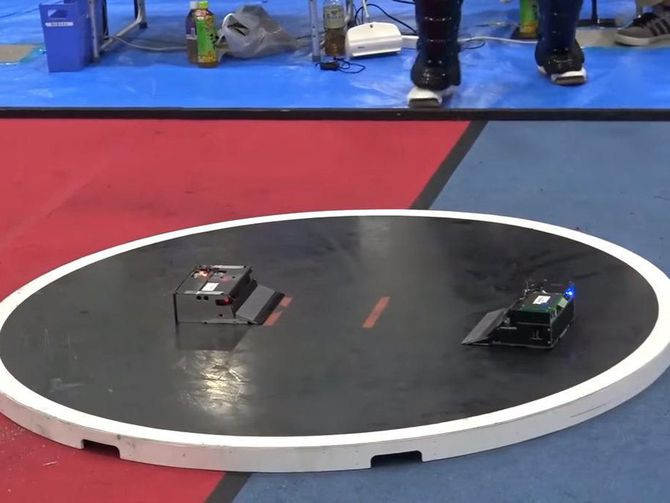
\includegraphics[width=0.75\linewidth]{pic01/sumo_competitions.jpg}
	\caption{Zawody sumo.}
	\label{fig:sumo_competitions}	
\end{figure}

\section{Założenia}
Główne założenia realizowanego projektu:
\begin{itemize}
\item stworzenie robota spełniającego wymagania kategorii minisumo,
\item sprawna sensoryka pozwalająca na wykrycie przeciwnika oraz końca ringu,
\item w pełni działająca komunikacja między robotem a aplikacją,
\item aplikacja mobilna pozwalająca na konfigurację wyżej wspomnianego robota.
\end{itemize}

Etapy realizacji wyżej wymienionych założeń zostały opisane w dalszej części pracy z podziałem na tworzonego robota minisumo oraz aplikację mobilną.

\chapter{Wykorzystane technologie}

Projekt został zrealizowany pod systemem Windows 10 oraz Mac OS X El Capitan. 

\section{C}
Z racji, iż sercem robota jest procesor z rodziny \textit{STM}, wybór technologii został ograniczony do języka C lub C++. Wybrano język C z powodów optymalizacyjnych oraz małego stopnia skomplikowania programu \cite{C}. 


Oprogramowanie zostało stworzone w środowisku \textit{Eclipse} z dodatkiem \textit{AC6} wspierającym platformę \textit{STM32}.

\subsection{Hardware Abstraction Layer}
\textit{HAL} jest biblioteką będącą wysokopoziomowym interfejsem służącym do konfiguracji peryferiów mikrokontrolera. Zdecydowano się na wyżej wspomnianą bilbiotekę z powodu bardzo przejrzystej dokumentacji oraz łatwości użytkowania. Dodatkowo użyto środowiska \textit{CubeMX}, które udostępnia graficzny interfejs pozwalający na stosunkowo łatwą oraz intuicyjną konfigurację procesora oraz wygenerowanie projektu w języku C wraz z~użyciem bibliotek HAL.

\newpage 

Rysunek ~\ref{fig:cubemx} przedstawia konfigurację peryferiów użytego procesora w środowisku CubeMX.   

\begin{figure}[H]
	\centering
		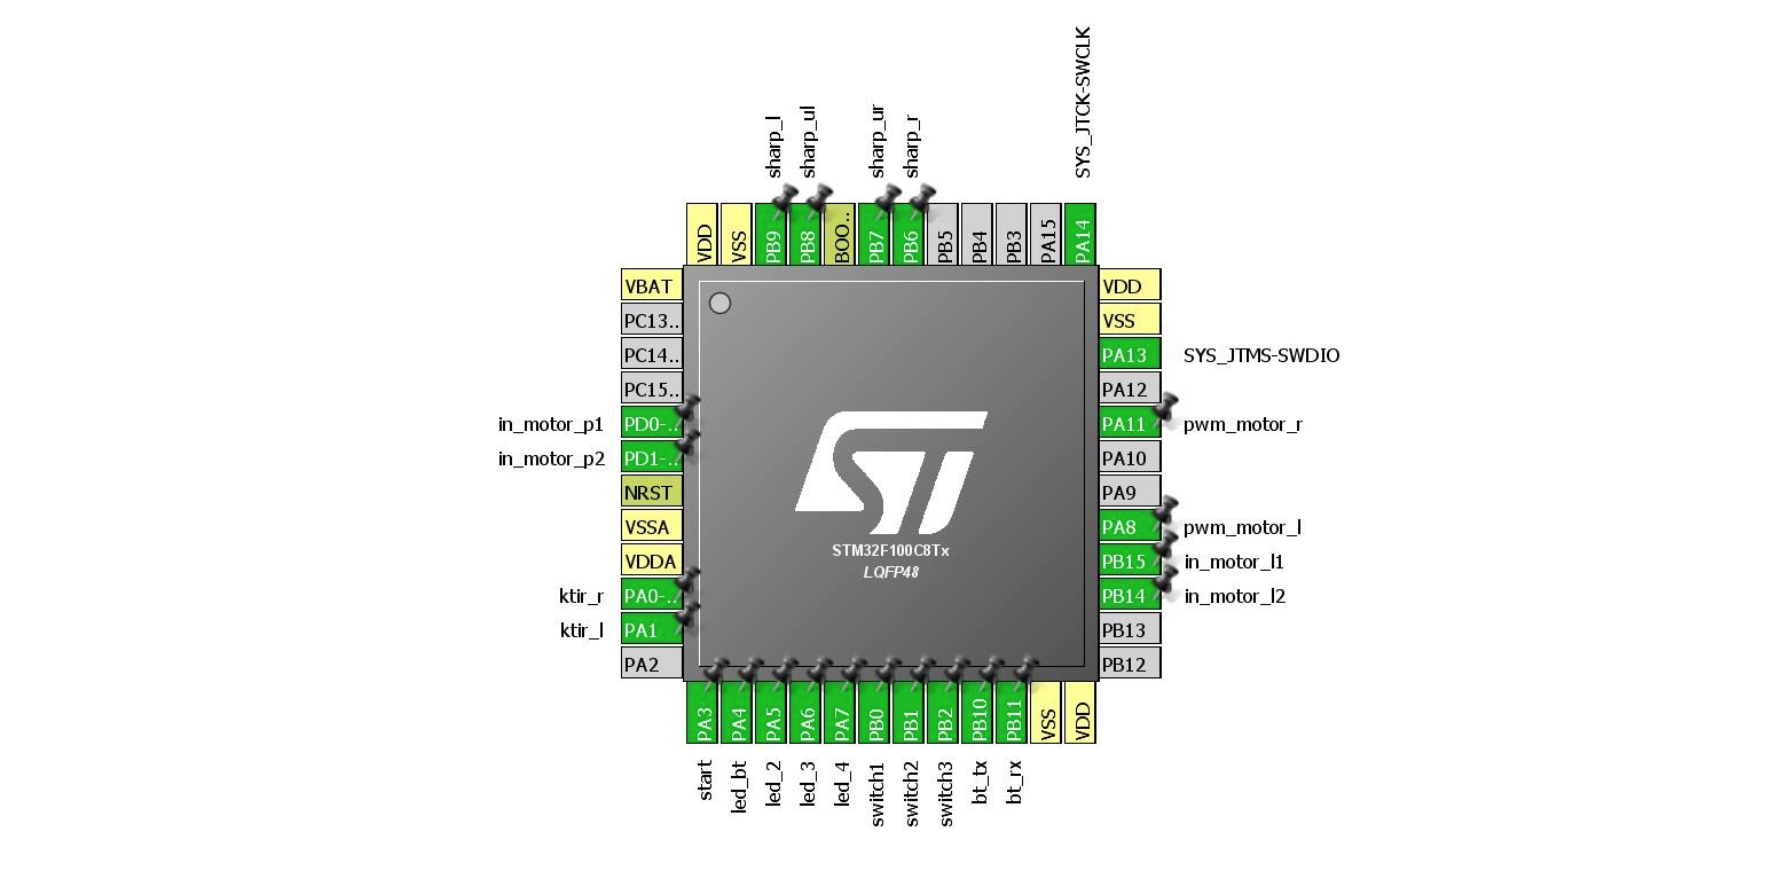
\includegraphics[width=\linewidth, scale=0.95]{pic02/cubemx}
	\caption{Konfiguracja peryferiów użytego procesora STM32F100C8T6B – LQFP48.}
	\label{fig:cubemx}	
\end{figure}

\newpage

\section{Swift}
\textit{Swift} jest językiem natywnym (następcą języka \textit{Objective–C}) zaprezentowanym przez \textit{Apple Inc.} w 2014 roku \cite{Swiftdoc}. Wykorzystywany jest do tworzenia oprogramowania na platformy \textit{macOS, iOS} oraz \textit{watchOS}. W pracy dyplomowej użyto wersji języka 3.0, ponieważ była to najnowsza wersja wspierana przez docelowe urządzenie, którym był telefon iPhone 5.

Środowiskiem użytym do tworzenia aplikacji mobilnej w technologii \textit{Swift} był \textit{Xcode}, którego dużym atutem jest występowanie graficznego interfejsu umożliwiającego tworzenie widoków aplikacji. Dzięki temu tworzenie aplikacji jest bardziej intuicyjne oraz pozwala na sprawne wprowadzanie zmian w tworzonych widokach \cite{Swift}.

Ilustracja ~\ref{fig:xcode} ukazuje środowisko Xcode wraz z widokami aplikacji oraz zależnościami między nimi.   

\begin{figure}[H]
	\centering
		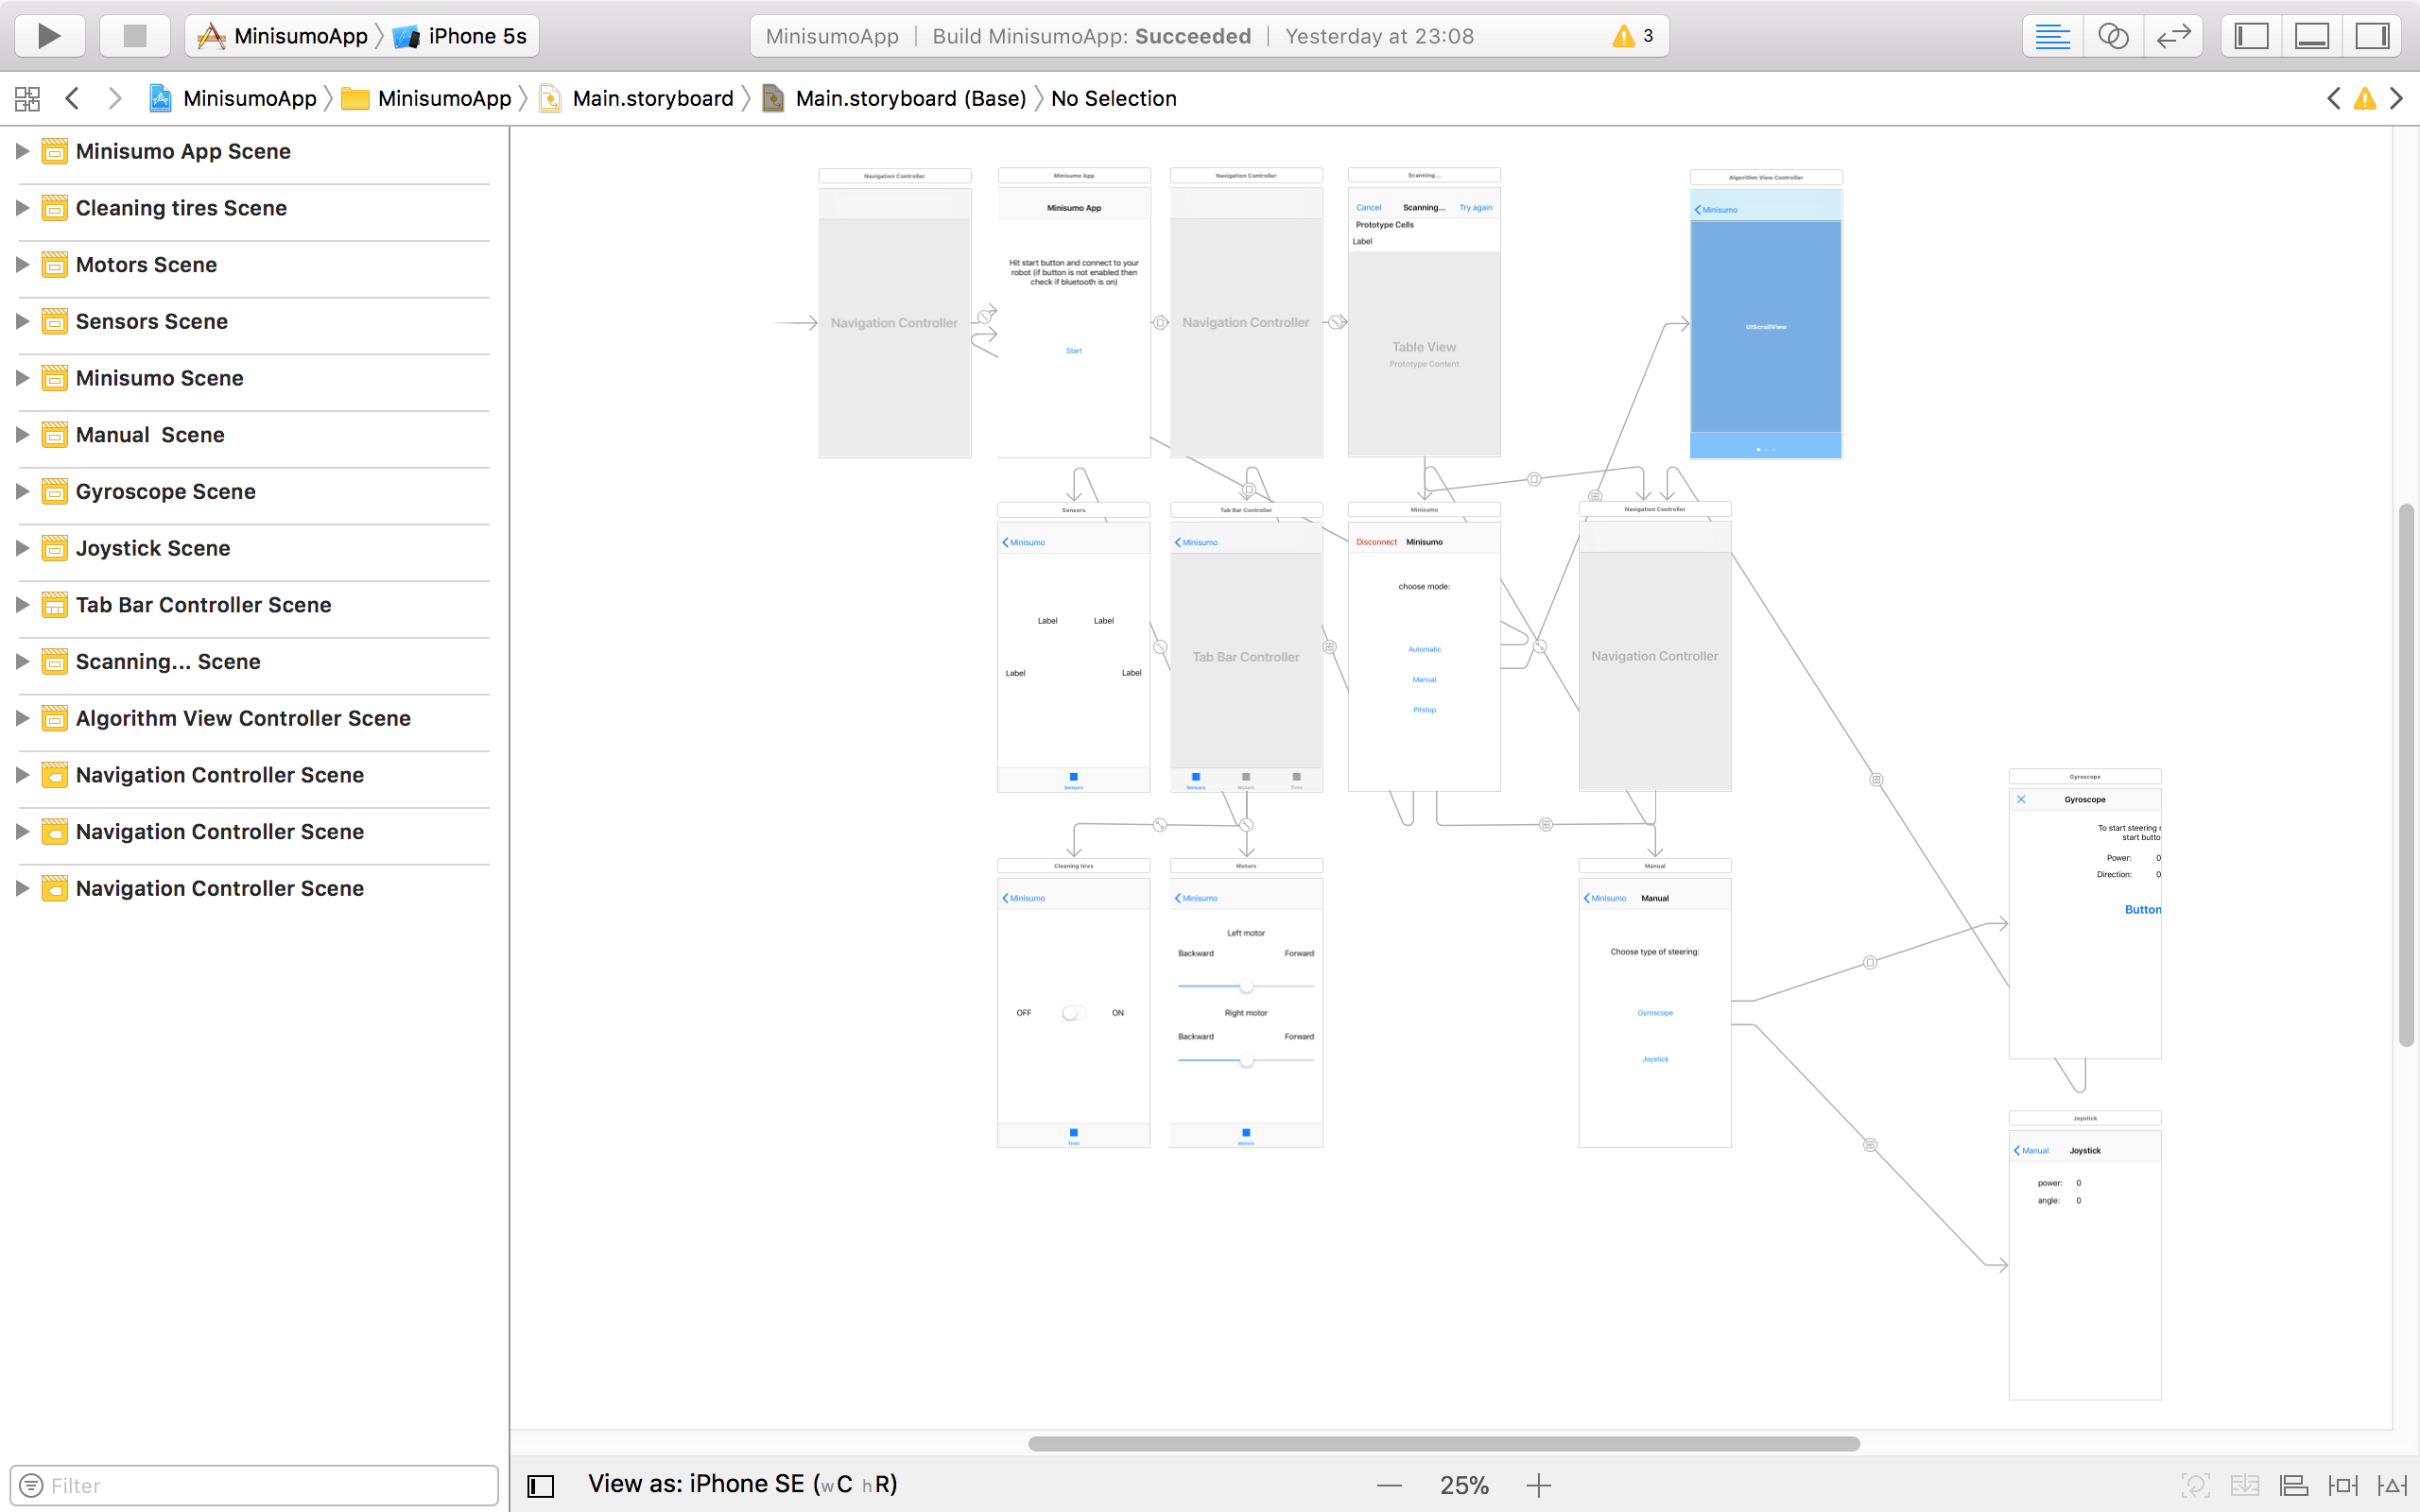
\includegraphics[width=0.75\linewidth]{pic02/xcode}
	\caption{Okno środowiska Xcode.}
	\label{fig:xcode}	
\end{figure}

\subsection{UIKit}
\textit{UIKit} jest platformą, która zapewnia infrastrukturę dla aplikacji. Udostępnia  architekturę widoku do implementacji interfejsu, obsługę zdarzeń, obsługę wielopunktowego dotyku, zarządza zasobami oraz interakcjami pomiędzy aplikacją a użytkownikiem. Dodatkowymi funkcjami są obsługa dokumentów, aplikacji oraz jej rozszerzeń, zarządzanie tekstem i wyświetlaniem \cite{AppleDocumentation}.

\index{UIView} \subsubsection{\lstinline$UIView$}
Widoki są podstawowymi elementami składowymi interfejsu użytkownika aplikacji, a klasa \textit{UIView} definiuje zachowania wspólne dla wszystkich widoków. Obiekt widoku renderuje zawartość w obrębie prostokąta obwiedni i obsługuje wszelkie interakcje z tą zawartością. 

\index{UITableView} \subsubsection{\lstinline$UITableView$}
\textit{UITableView} wyświetla listę pozycji w pojedynczej kolumnie. Jest podklasą \textit{UIScrollView}, która pozwala użytkownikowi przewijać tabelę, z tą różnicą, że przewijanie dozwolone jest wyłącznie w pionie. Komórki zawierające poszczególne elementy tabeli są obiektami \textit{UITableViewCell}. \textit{UITableView} używa wspomnianych obiektów do rysowania widocznych wierszy tabeli. Komórki mogą posiadać tytuły treści, obrazy oraz widoki akcesoriów, które mogą pełnić rolę elementów sterujących takich jak przełączniki i suwaki. 

\subsection{CoreBluetooth}
Platforma \textit{CoreBluetooth} dostarcza klasy niezbędne do komunikacji aplikacji z urządzeniami wyposażonymi w bezprzewodową komunikację Bluetooth.

\index{CBPeripheral} \subsubsection{\lstinline$CBPeripheral$}
Klasa \textit{CBPeripheral} reprezentuje zdalne urządzenia peryferyjne, których połączenie  aplikacja wykrywa za pośrednictwem instancji \textit{CBCentralManager}. Urządzenia peryferyjne są identyfikowane za pomocą unikalnych identyfikatorów (UUID) reprezentowanych przez obiekty NSUUID. 

\index{CBCentralManager} \subsubsection{\lstinline$CBCentralManager$}
Obiekty \textit{CBCentralManager} służą do zarządzania podłączonymi urządzeniami peryferyjnymi (reprezentowanymi przez obiekty \textit{CBPeripheral}). Pozwalają na skanowanie oraz wykrywanie zdalnych urządzeń.

\subsection{CoreGraphics}
Platforma \textit{CoreGraphics} oparta jest na zaawansowanym mechanizmie rysowania \textit{Quartz}. Zapewnia niskopoziomowe renderowanie 2D, zarządzanie wzorcami, gradientami oraz danymi obrazu. Dodatkowo pozwala na tworzenie oraz maskowanie obrazu, a także wyświetlanie i analizowanie dokumentów PDF. W pracy dyplomowej \textit{CoreGrapics} zostało wykorzystane do stworzenia wirtualnego dżojstiku służącego zdalnemu sterowaniu robotem minisumo. 

\subsection{CoreMotion}
Dostarcza dane dotyczące ruchu urządzenia na podstawie wbudowanego akcelerometru, żyroskopu, krokomierza, magnetometru, barometru itp. W aplikacji użyto wspomnianej platformy do sterowania ruchem robota za pomocą akcelerometru \cite{AppleDocumentation}.

\section{Arduino}
\textit{Arduino} jest platformą programistyczną przeznaczoną dla mikrokontrolerów z wbudowaną obsługą układów wejścia oraz wyjścia \cite{Arduino}. Język programowania \textit{Arduino} oparty jest na języku C/C++. Głównym atutem omawianej platformy jest szeroka społeczność, dokładna dokumentacja oraz łatwość prototypowania prostych układów. Jednakże omawiania platfomra nie jest zalecana w~przypadku złożonych projektów ze względu na wysokopoziomowość oraz niestabilność pracy.

Platforma została użyta do konfiguracji modułu Bluetooth za pomocą komend \textit{AT}. Skonfigurowano takie parametry jak nazwa urządzenia oraz liczbę symboli na sekundę (ang. \textit{baud rate}). Do tego celu użyto mikrokontrolera \textit{Arduino Mega 2560} oraz płytki stykowej wraz z przewodami połączeniowymi. Konfiguracja modułu była jednorazową czynnością, dlatego zdecydowano się na platformę \textit{Arduino} ze względu na wyżej wspomnianą szybkość oraz prostotę obsługi.
  

\begin{figure}[H]
	\centering
		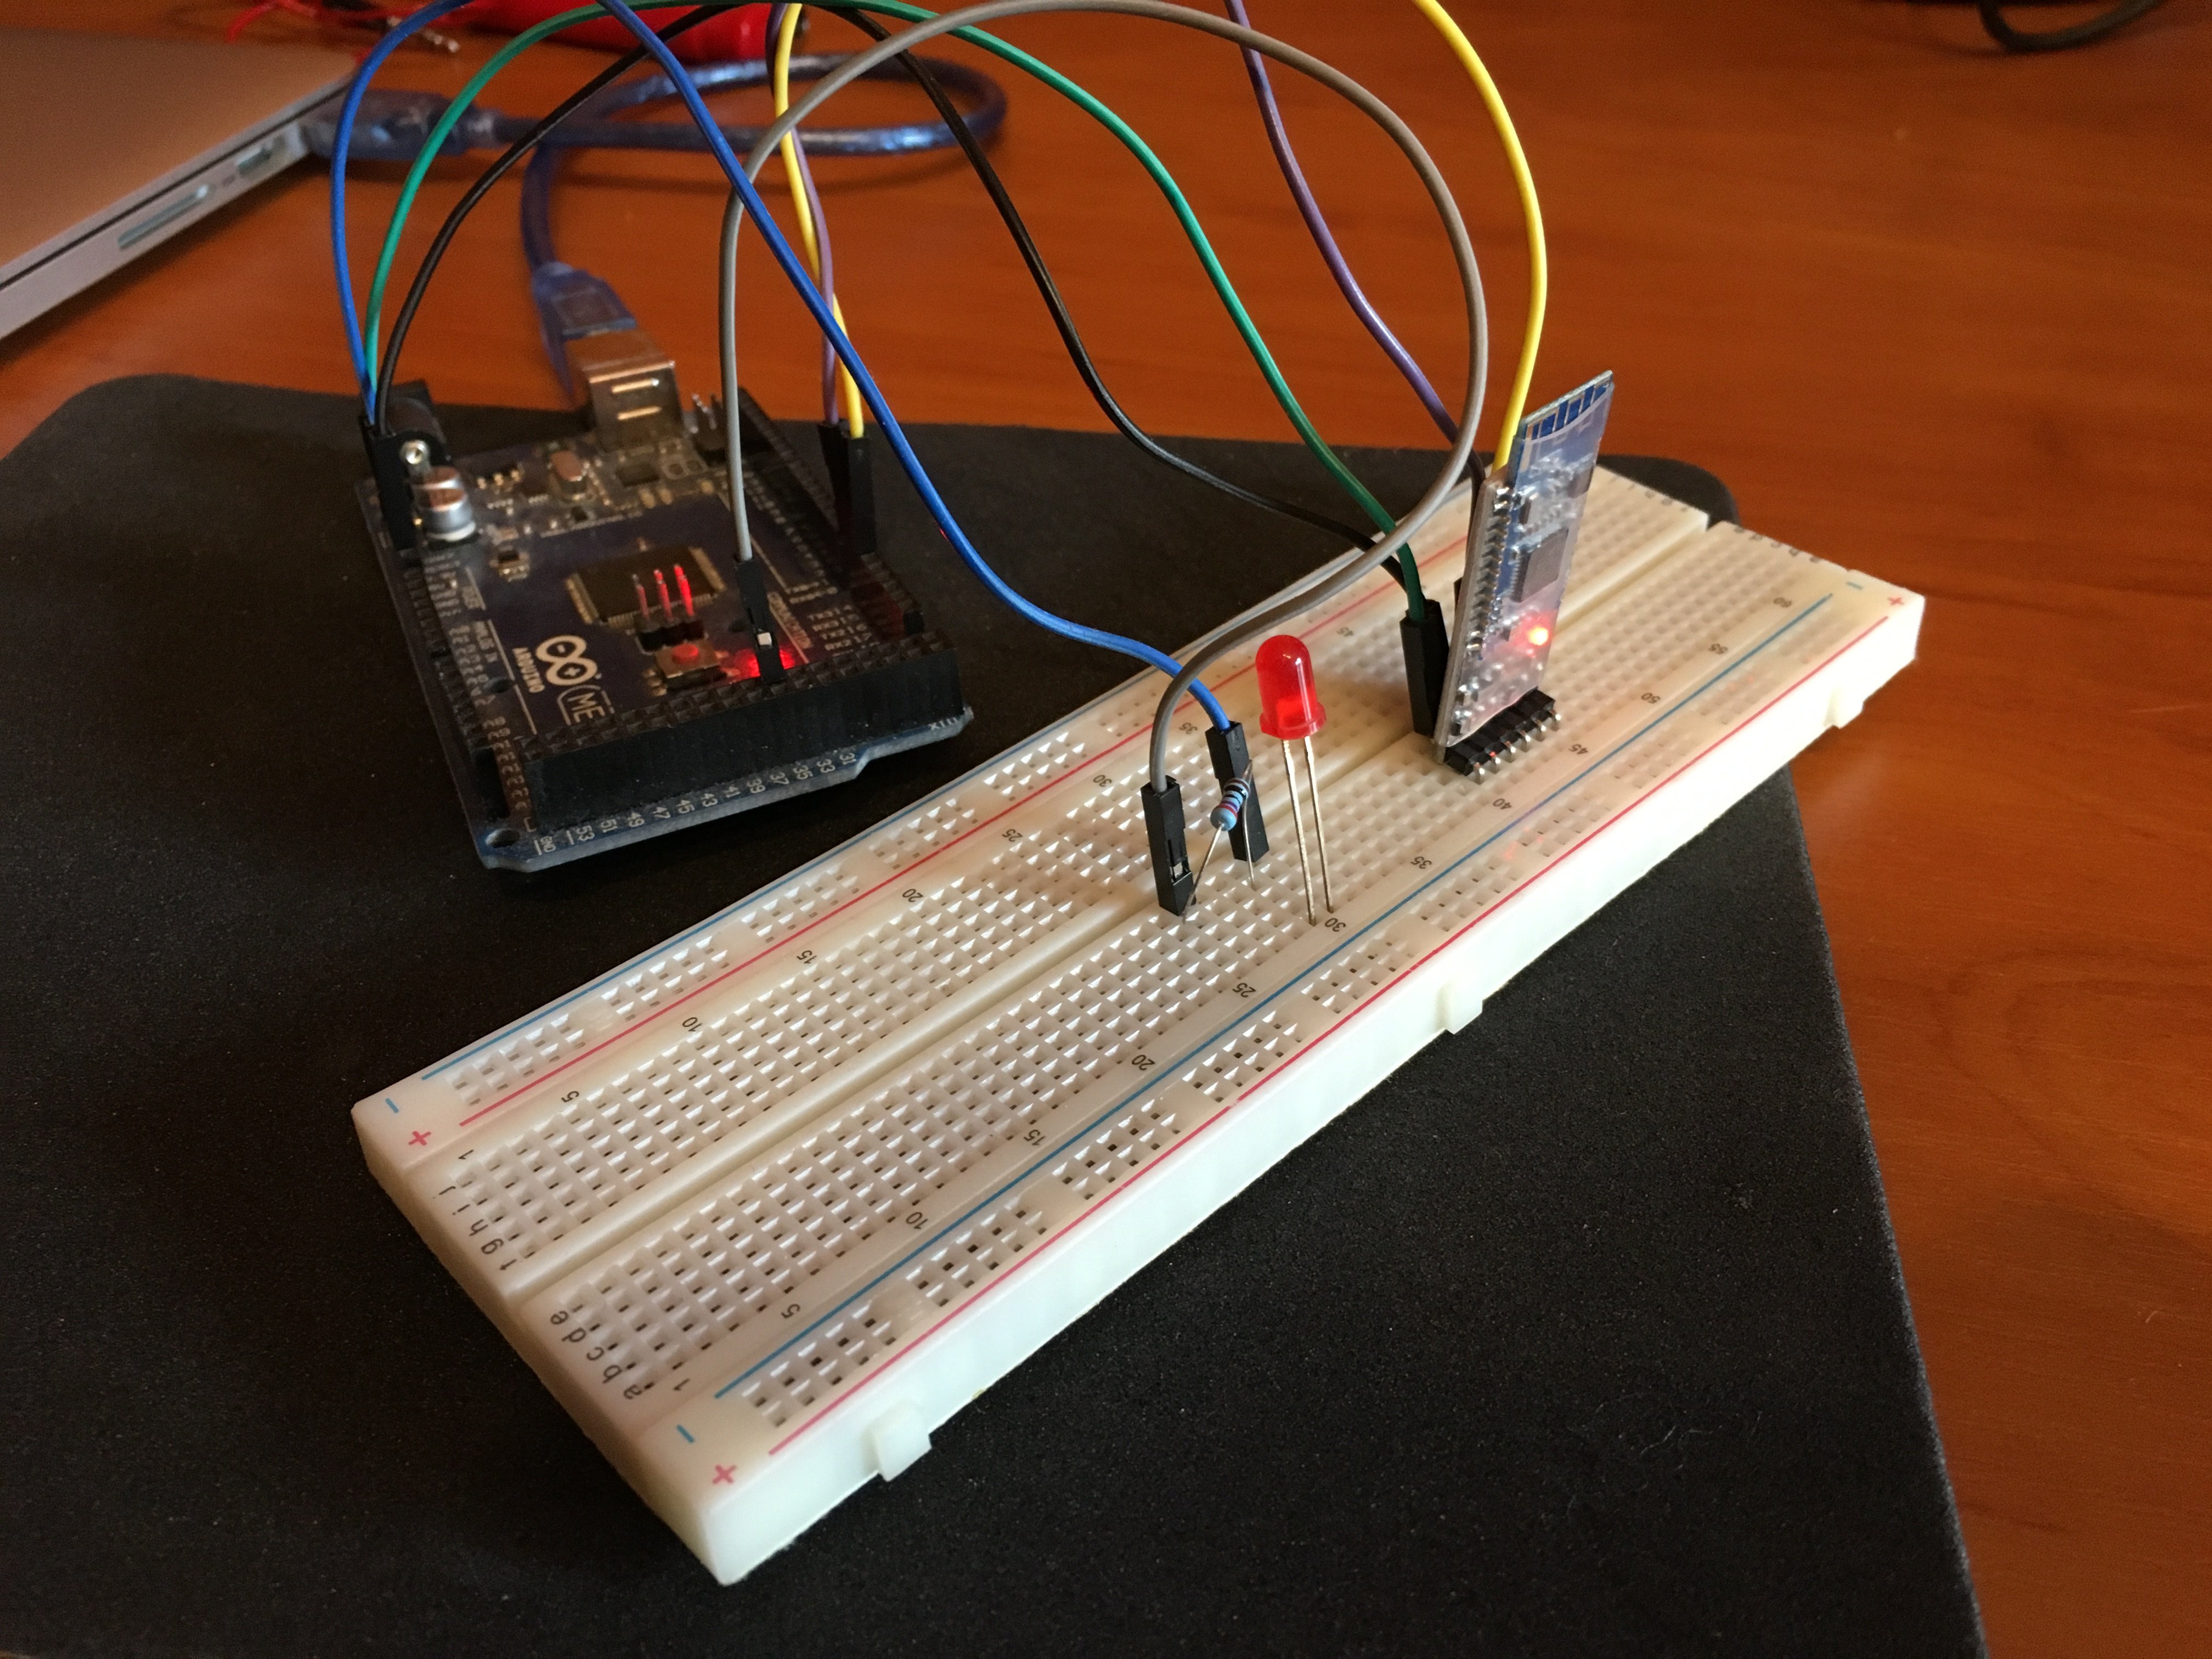
\includegraphics[width=0.75\linewidth]{pic02/arduino.JPG}
	\caption{Układ służący do konfiguracji modułu bluetooth.}
	\label{fig:arduino}	
\end{figure}

Rysunek ~\ref{fig:arduino} obrazuje układ \textit{Arduino Mega 2560} wraz z płytką stykową oraz podłączonym modułem bluetooth. Dodatkowo układ wyposażono w diodę mającą na celu sygnalizację poprawności wgrywania komend.

\newpage 

Listing \ref{arduinocode} przedstawia kod programu zapewniającego komunikację między komputerem a~modułem Bluetooth przy użyciu mikrokontrolera \textit{Arduino Mega 2560}. 

\begin{minipage}{\textwidth}
	\begin{lstlisting}[label=arduinocode,caption=Kod programu umożliwiającego konifugrację modułu Bluetooth HM–10.]
#include <SoftwareSerial.h>
 
int LEDPIN = 13;

void setup() {
  pinMode(LEDPIN, OUTPUT);
  Serial.begin(9600); // communication with computer
  Serial3.begin(9600); // communication with HM-10  
}
 
void loop() {
  if ( Serial3.available() ) {
    char dioda = Serial3.read();
    Serial.write(dioda);
    if (atoi(&dioda)==1) {
      digitalWrite(LEDPIN, HIGH);
    }
    
    if (atoi(&dioda)==0) {
      digitalWrite(LEDPIN, LOW);
    }
  }
  
  if ( Serial.available() ) {  Serial3.write( Serial.read() );  }  
}
	\end{lstlisting}
\end{minipage}
 
Za pomocą terminalu udostęnionego przez środowisko \textit{Arduino} możliwa jest komunikacja oraz konfiguracja modułu \textit{HM–10}. Dodatkowo program został rozszerzony o zapalanie oraz gaszenie diody LED w celu sprawdzenia poprawności połączenia. Jeżeli przy użyciu wyżej wspomnianego terminala zostanie wysłana wartość 1, powinna zapalić się dioda. W przypadku wysłania wartości 0, dioda powinna zgasnąć.


 

\chapter{Komunikacja}
Komunikacja między urządzeniami (robotem a aplikacją mobilną) została zrealizowana przy użyciu łączności bezprzewodowej Bluetooth. 

\begin{figure}[H]
	\centering
		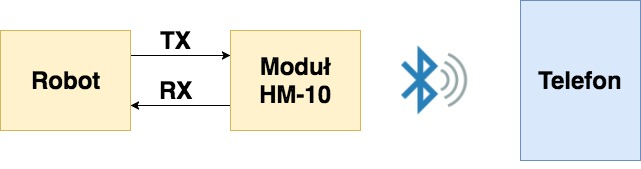
\includegraphics[width=0.75\linewidth]{pic03/bt_communications.jpg}
	\caption{Schemat komunikacji między urządzeniami.}
	\label{fig:communication}	
\end{figure}

Na rysunku ~\ref{fig:communication} przedstawiono schemat komunikacji między robotem a aplikacją mobilną. Aplikacja mobilna komunikuje się radiowo z modułem Bluetooth, który następnie za pomocą przewodów podłączonych do linii TX oraz RX procesora przesyła wysłaną wiadomość.   

\section{Moduł bluetooth}
Z racji, iż docelowym urządzeniem komunikującym się z robotem był telefon iPhone, który obsługuje wyłącznie technologię BLE (Bluetooth Low Energy), wybór docelowego modułu komunikacyjnego został mocno ograniczony. Z początku zdecydowano się na moduł Bluetooth HM–11 ze względu na bardzo małe rozmiary. Niestety okazało się, iż owy moduł posiada nietypowy raster, przez co niemożliwym było przylutowanie jakiegokolwiek złącza. Jedynym rozwiązaniem byłoby przylutowanie modułu do płytki elektronicznej robota, aczkolwiek projekt płytki nie przewidywał dodatkowych elementów. W związku z czym zdecydowano się na starszy model HM–10, który dostarczał taką samą funkcjonalność, lecz posiadał gotowe złącze goldpin, które znacząco ułatwiło podłączenie do wyżej wspomnianej płytki. Jedyną wadą zastosowanego modułu był rozmiar.

\begin{figure}[H]
	\centering
		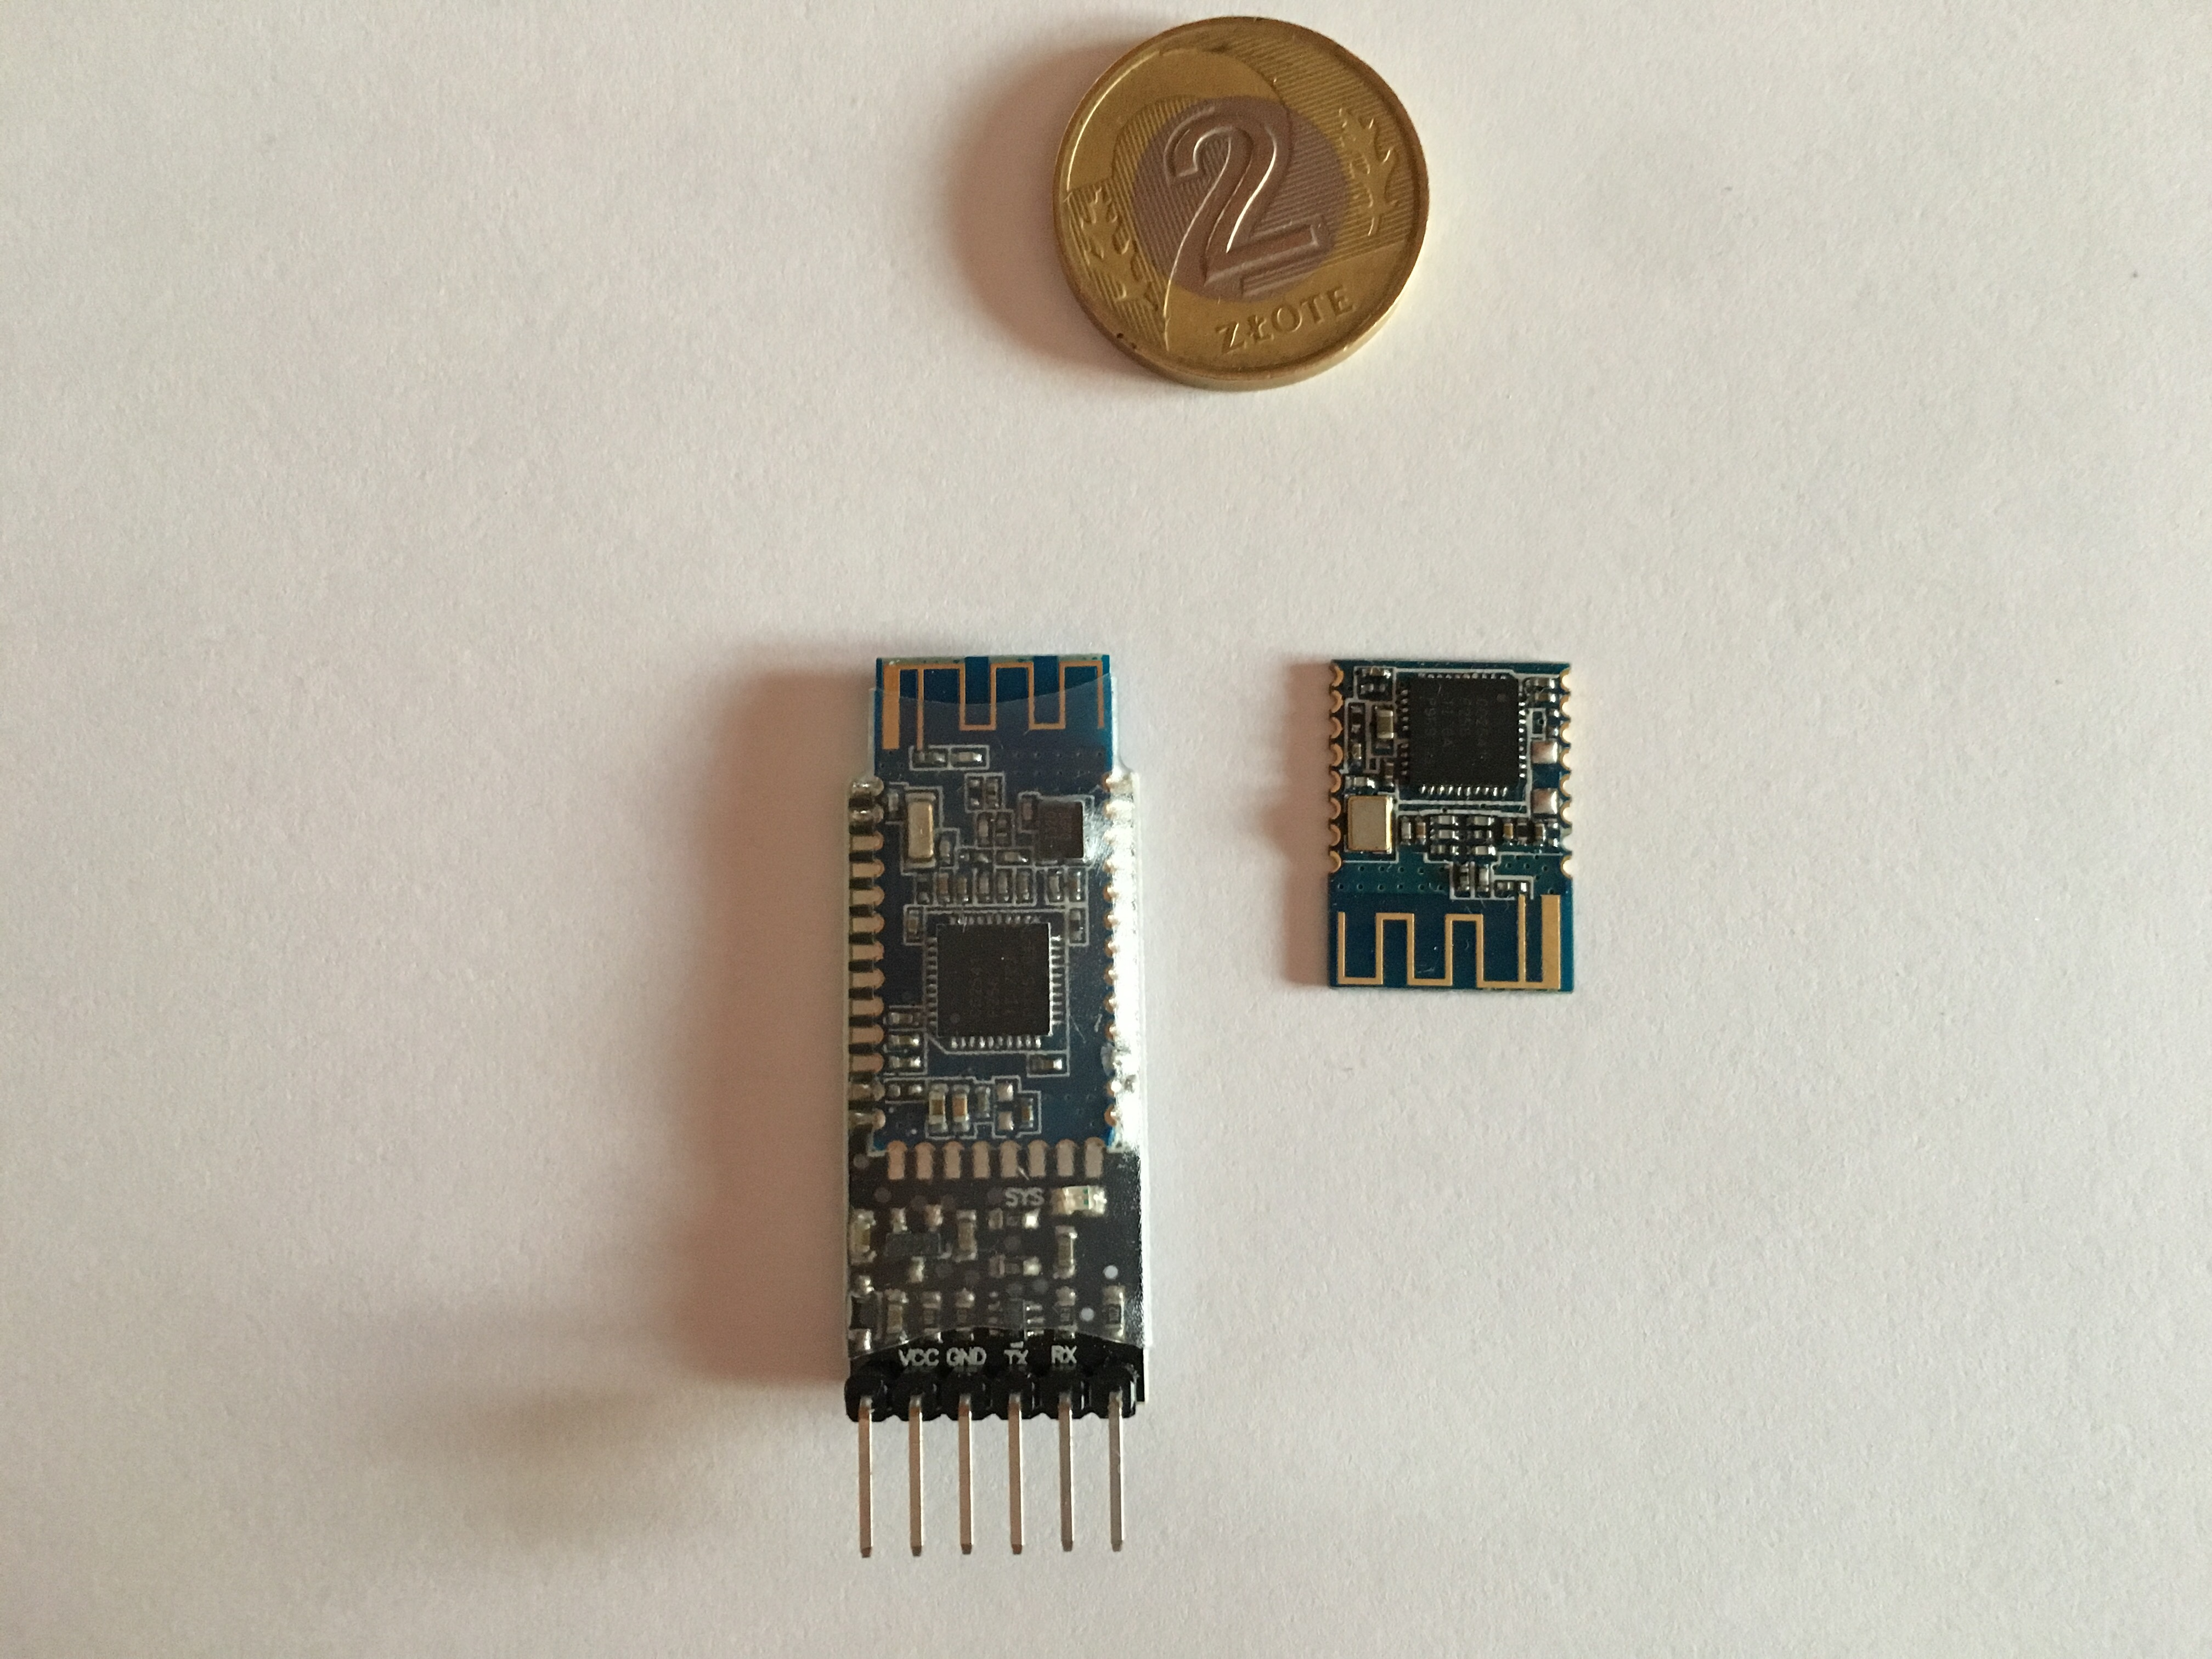
\includegraphics[width=0.75\linewidth]{pic03/bt_modules.jpg}
	\caption{Moduły Bluetooth.}
	\label{fig:bt}	
\end{figure}

Na rysunku ~\ref{fig:bt} po lewej stronie widoczny jest docelowo użyty moduł HM–10, natomiast po prawej wcześniej wspomniany HM–11. U góry ilustracji znajduję się moneta dla odwzorowania rozmiarów omawianych układów.

\section{Realizacja komunikacji}
Komunikacja między urządzeniami bazuje na wysyłaniu ciągu dziesięciu znaków, a dokładniej nieujemnych liczb całkowitych, które następnie są parsowane oraz interpretowane w odpowiedni sposób. Domyślnie wiadomość składa się z dziesięciu zer, a następnie wypełniana jest odpowiednimi wartościami. Poniżej przedstawiono przykładowe formaty wiadomości przesyłane między urządzeniami.

\index{Sensory} \subsubsection{\lstinline$Sensory$}
Komunikacja między urządzeniami rozpoczyna się od wysłania wiadomości przez aplikację mobilną w której pierwsza cyfra wiadomości ma wartość równą 4. Następnie co określony czas robot wysyła wiadomość w której zawarty jest aktualny stan czujników. Komunikacja kończy się w momencie, gdy aplikacja mobilna wyśle wiadomość w której pierwsza cyfra jest różna od 4.

\begin{figure}[H]
	\centering
		
\includegraphics[width=0.75\linewidth]{pic03/sensors.jpg}
	\caption{Schemat wiadomości zawierającej informacje odnośnie stanu sensorów.}
	\label{fig:sensors_communication}	
\end{figure}

Na rysunku ~\ref{fig:sensors_communication} przedstawiono strukturę wiadomości wysłanej przez robota do aplikacji mobilnej. Pierwsza cyfra (równa 4) sygnalizuje aplikacji, iż przesyłana wiadomość zawiera informacje na temat stanu czujników. Cyfry \textit{A, B, C, D} sygnalizują stan cyfrowych czujników wykrywających przeciwnika w sposób binarny (0 – nie wykryto przeciwnika, 1 – wykryto przeciwnika). Cyfry \textit{XX} oraz \textit{YY} informują o stanie analogowych czujników wykrywających koniec ringu (00 – wykryto czarny kolor, 99 – wykryto biały kolor).

\index{Automatyczne sterowanie} \subsubsection{\lstinline$Automatyczne Sterowanie$}

Komunikacja bazuje na jednorazowym wysłaniu wiadomości do robota z poziomu aplikacji mobilnej. Treść wiadomości określa czy robot powinien wstrzymać start do momentu otrzymania komunikatu od sędziego, rodzaj algorytmu walki oraz maksymalną moc silników.

\begin{figure}[H]
	\centering
		
\includegraphics[width=0.75\linewidth]{pic03/automatic.jpg}
	\caption{Schemat wiadomości w której zawarta jest konfiguracja robota.}
	\label{fig:automatic}	
\end{figure}

Rysunek ~\ref{fig:automatic} obrazuje schemat wiadomości wysłanej z aplikacji mobilnej do robota. Pierwsza cyfra (równa 1) informuje, iż robot przechodzi w stan automatycznej jazdy. Cyfra \textit{A} określa numer algorytmu walki (na chwilę obecną występują trzy algorytmy, numerowane 1,2 oraz 3). Kolejna cyfra \textit{B} dostarcza informację odnośnie rodzaju startu (0 – ruch robota rozpoczyna się w~momencie wysłania wiadomości, 1 – robot oczekuje na sygnał sędziego). Ostatnia wartość \textit{XXX} określa procentowo maksymalną moc jaką mogą osiągnąć obydwa silniki (przyjmuje wartości 000 – 100, gdzie 100 oznacza maksymalną moc, a 000 minimalną).

\index{Sterowanie zdalne – akcelerometr} \subsubsection{\lstinline$Sterowanie zdalne - akcelerometr$}

Aplikacja mobilna jednorazowo wysyła komunikat, którego pierwsza cyfra oznacza wejście w~tryb zdalnego sterowania. Następnie wspomniana aplikacja rozpoczyna nasłuchiwanie wiadomości zawierających kierunki ruchu oraz moce poszczególnych silników wysyłanych przez robota.

\begin{figure}[H]
	\centering
		
\includegraphics[width=0.75\linewidth]{pic03/accelerometer.jpeg}
	\caption{Schemat wiadomości zdalnego sterowania przy użyciu akcelerometru.}
	\label{fig:accelerometer}	
\end{figure}

Ilustracja ~\ref{fig:accelerometer} przedstawia budowę wiadomości wysłanej do aplikacji mobilnej przez robota. Pierwsza cyfra (równa 6) wskazuje, iż robot jest w trybie zdalnego sterowania za pomocą akcelerometru. Kolejne cyfry \textit{A} oraz \textit{B} oznaczają kierunki odpowiedno lewego oraz prawego silnika (1 – obrót w tył, 2 – obrót w przód). \textit{XXX} oraz \textit{YYY} podobnie jak w przypadku trybu automatycznej jazdy określają procentowe moce silników, lewego oraz prawego (przyjmują wartości 000 – 100, gdzie 100 oznacza maksymalną moc, a 000 minimalną).  


\chapter{Robot minisumo}

W niniejszym rozdziale opisany został proces tworzenia robota minisumo. Wyróżniono w nim trzy główne sekcje: \textit{Konstrukcja}, \textit{Elektronika} oraz \textit{Oprogramowanie}.

\begin{figure}[H]
	\centering
		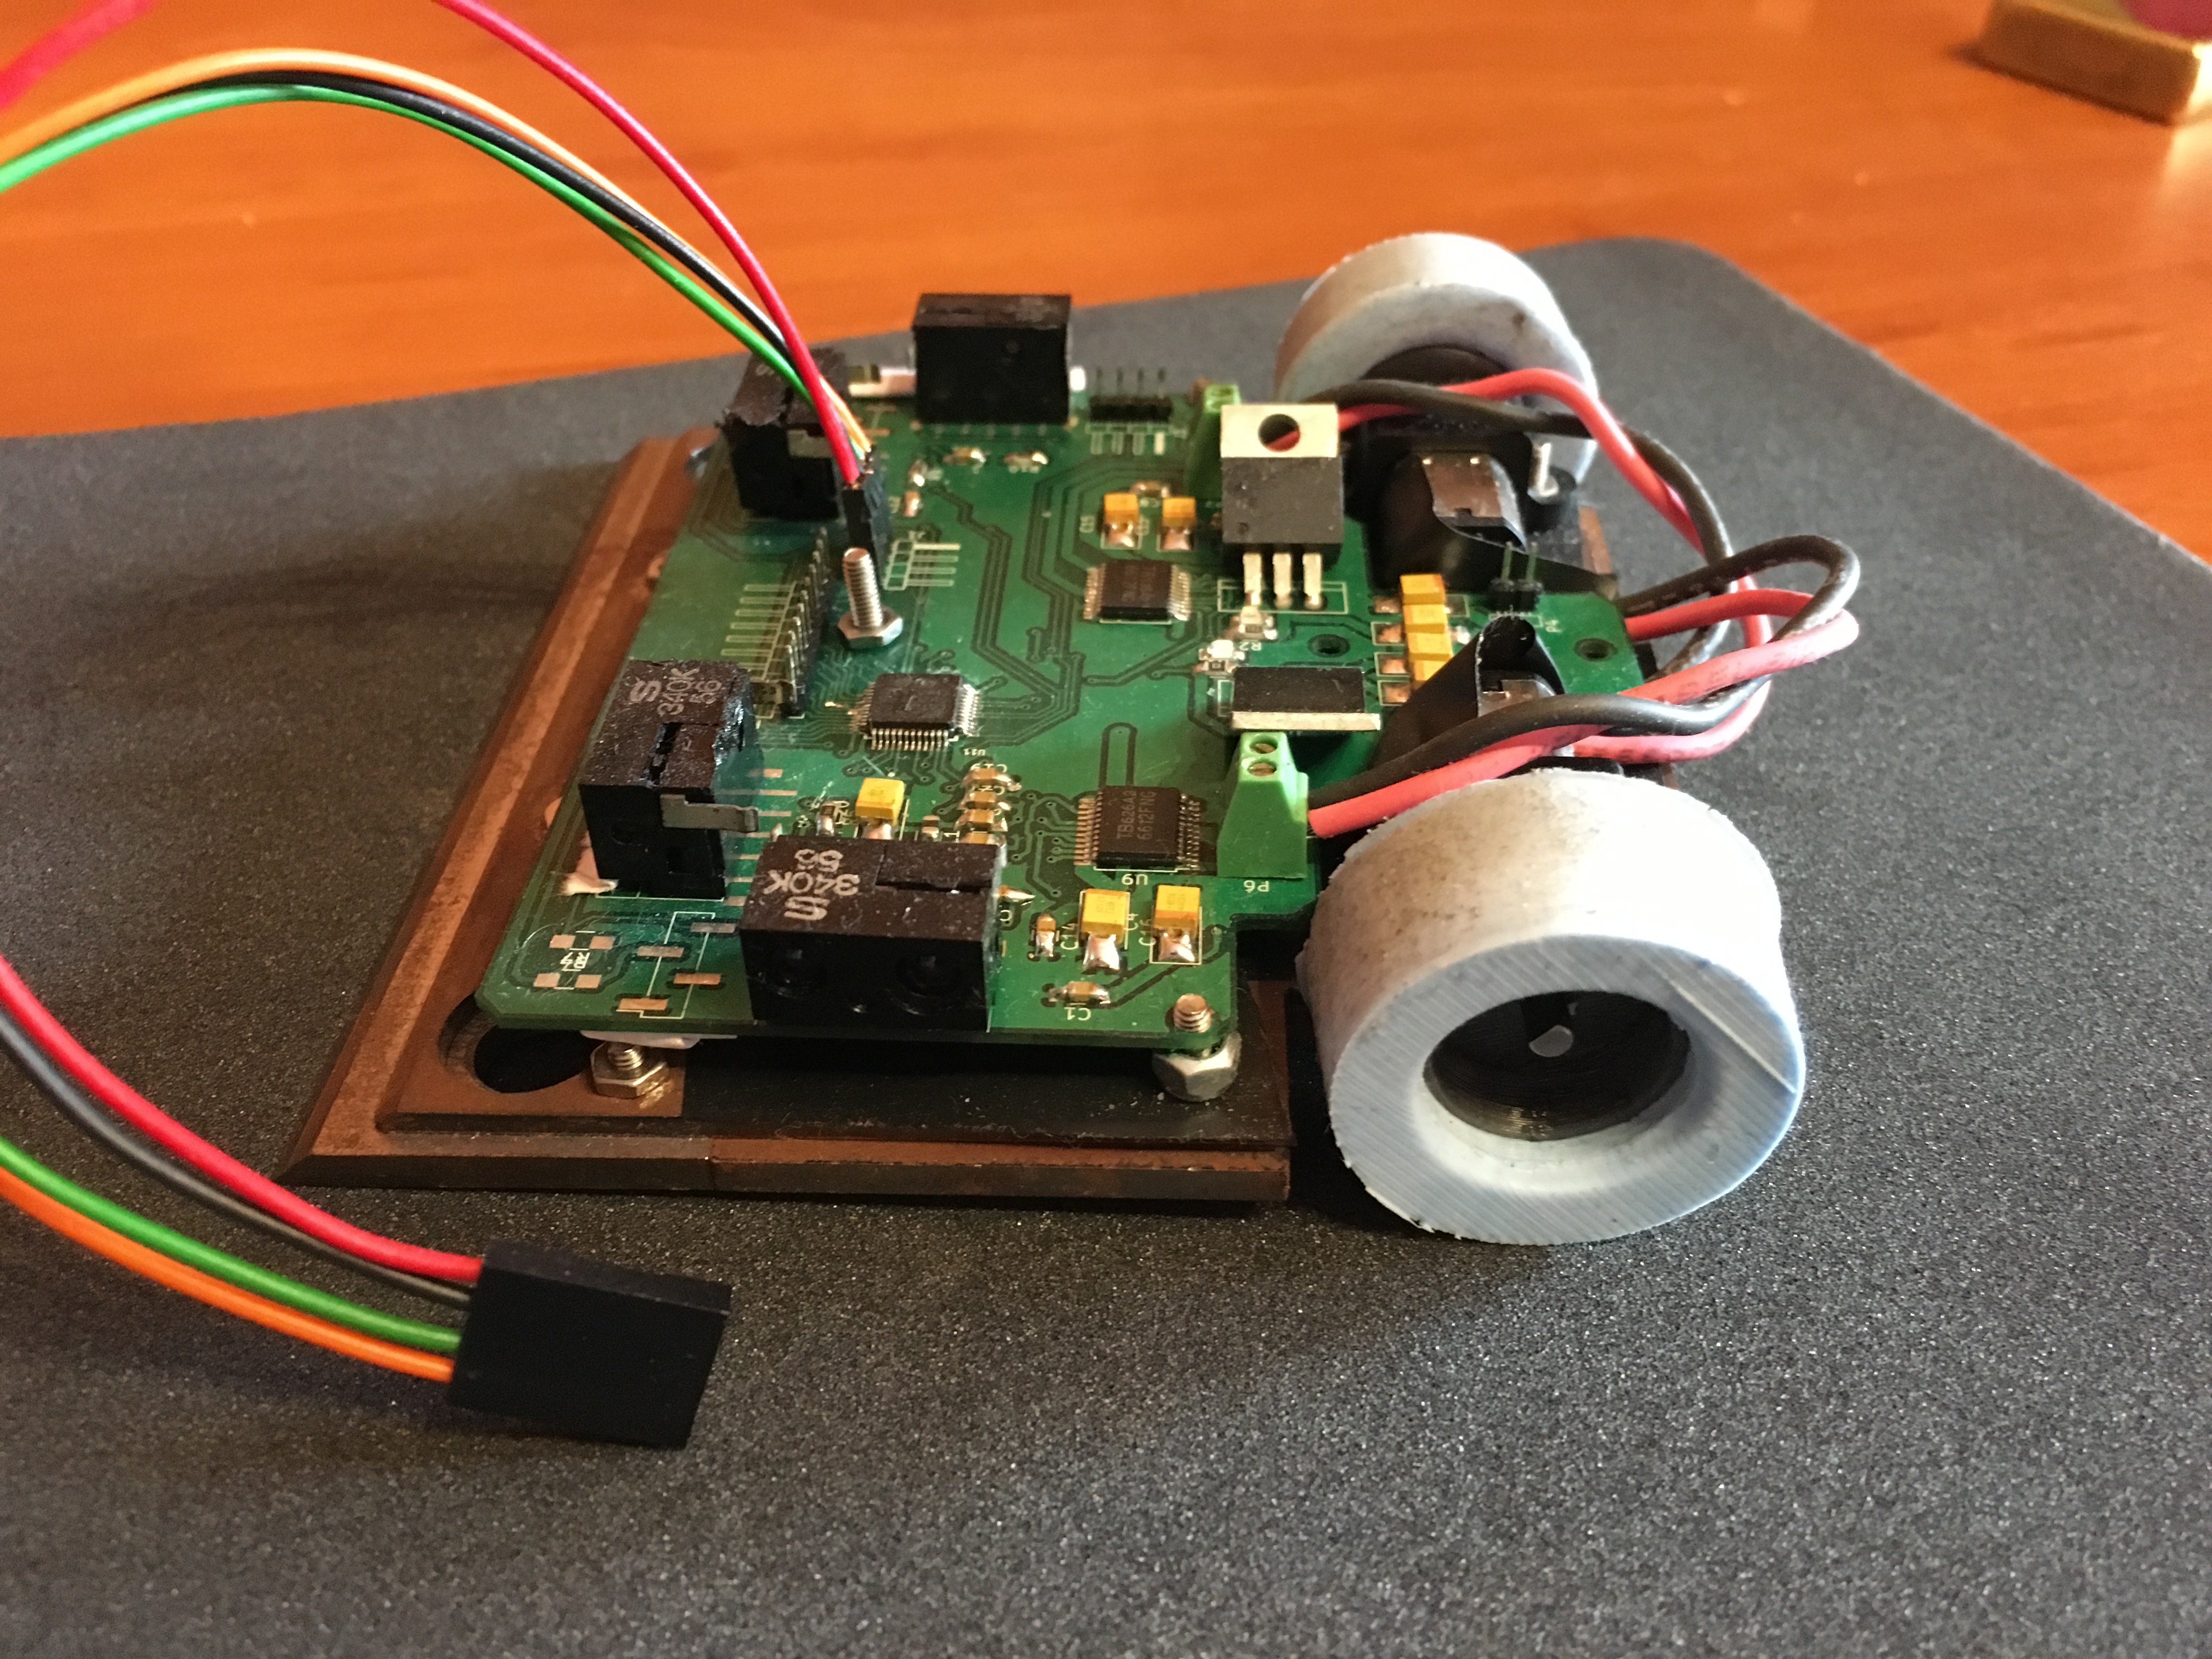
\includegraphics[width=0.75\linewidth]{pic04/minisumo.JPG}
	\caption{Wykonany robot minisumo.}
	\label{fig:robot}	
\end{figure}

Rysunek ~\ref{fig:robot} przedstawia omawianego robota minisumo. W celu ukazania elektroniki ściągnięto nadwozie.

\newpage 

\section{Konstrukcja}
\subsection{Założenia}
Głównym założeniem konstrukcyjnym było zminimalizowanie szansy podbicia robota przez przeciwnika. W związku z czym napęd robota składa się z dwóch kół umiejscowionych w tylnej części konstrukcji. Przednia część robota zakończona jest pługiem, który bezpośrednio dotyka podłoża. Dodatkowo starano się, aby środek ciężkości całej konstrukcji znajdował się jak najbliżej podłoża.

\subsection{Nadwozie}
Konstrukcja nadwozia została zaprojektowana przy użyciu środowiska \textit{Autodesk Inventor 2017}. Wybór został podyktowany łatwością obsługi narzędzi oraz darmową licencją studencką. Obudowa została wykonana w technologii druku 3D, ze względu na małą masę, koszt produkcji oraz możliwość łatwego dostosowania do potrzeb projektu (otwory na śruby oraz czujniki przeciwnika, przestrzeń na koła).  

\begin{figure}[H]
	\centering
		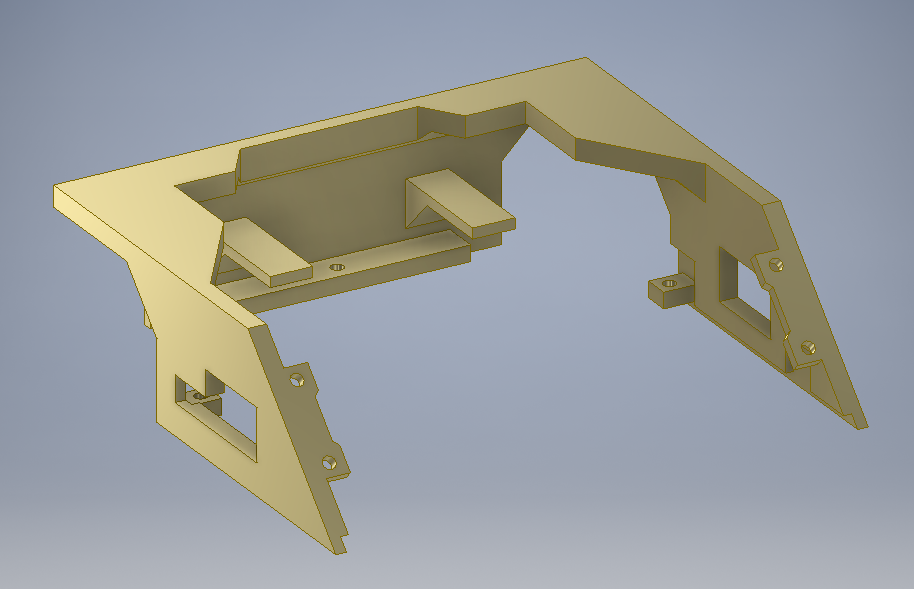
\includegraphics[width=0.75\linewidth]{pic04/body.png}
	\caption{Projekt nadwozia w środowisku Autodesk Inventor 2017.}
	\label{fig:body}	
\end{figure}

Na rysunku ~\ref{fig:body} przedstawiono projekt nadwozia robota. Ze względu na niewielką wytrzymałość plastikowego wydruku przywiązano dużą wagę do szerokości obudowy. Starano się, aby była możliwie jak najszersza, co skutkowało wzrostem trwałości całej konstrukcji. Dodatkowo front robota został wykonany ze stali, ponieważ w przypadku podważenia przeciwnika jest obszarem najbardziej podatnym na zniszczenia. 

\newpage

\subsection{Podwozie}
Całość podwozia wykonana została ze stali ze względu na wytrzymałość oraz dużą masę, która przyczyniła się do znacznego obniżenia środka ciężkości konstrukcji.  Podobnie jak w przypadku nadwozia projekt został stworzony w środowisku \textit{Autodesk Inventor 2017}. Konstrukcja składa się z trzech płytek, z czego jedna zawiera ostrze od strugarki, wykonane z węglika spiekanego. Materiał ten cechuje się wysoką wytrzymałością oraz większą odpornością na kruszenie w porównaniu do zwykłej stali. 

\begin{figure}[H]
	\centering
		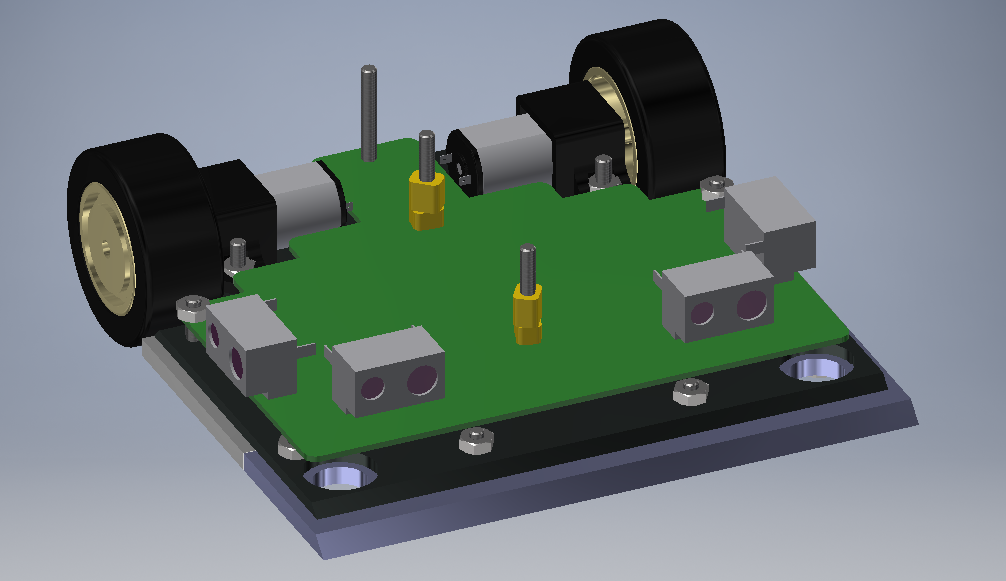
\includegraphics[width=0.75\linewidth]{pic04/chassis.png}
	\caption{Projekt podwozia w środowisku Autodesk Inventor 2017.}
	\label{fig:chassis}	
\end{figure}

Rysunek ~\ref{fig:chassis} ukazuje wizualizację podwozia wraz z silnikami oraz kołami. Projekt wyeksportowano do formatu 2D, a następnie wykonano przy użyciu techniki wypalania laserem. 

\subsection{Napęd}
Jak wspomniano wcześniej, napęd robota składa się z dwóch kół, które sterowane są niezależnie. Ruch robota wzorowany jest na zasadzie działania czołgu. W przypadku skrętu, do jednego z silników dostarczana jest większa moc, co skutkuje wzrostem prędkości kątowej napędzanego koła. Z powodu różnicy prędkości kół robot zaczyna skręcać. Zdecydowano się na takie rozwiązanie ze względu na dozwoloną masę (większa ilość kół oraz silników znacząco by ją zwiększyła) oraz manewrowość – dzięki zastosowaniu omawianego rozwiązania możliwy jest obrót robota w miejscu (w przypadku, gdy koła kręcą się w przeciwne strony), dzięki czemu pojazd jest szybki oraz zwinny. 

\begin{figure}[H]
	\centering
		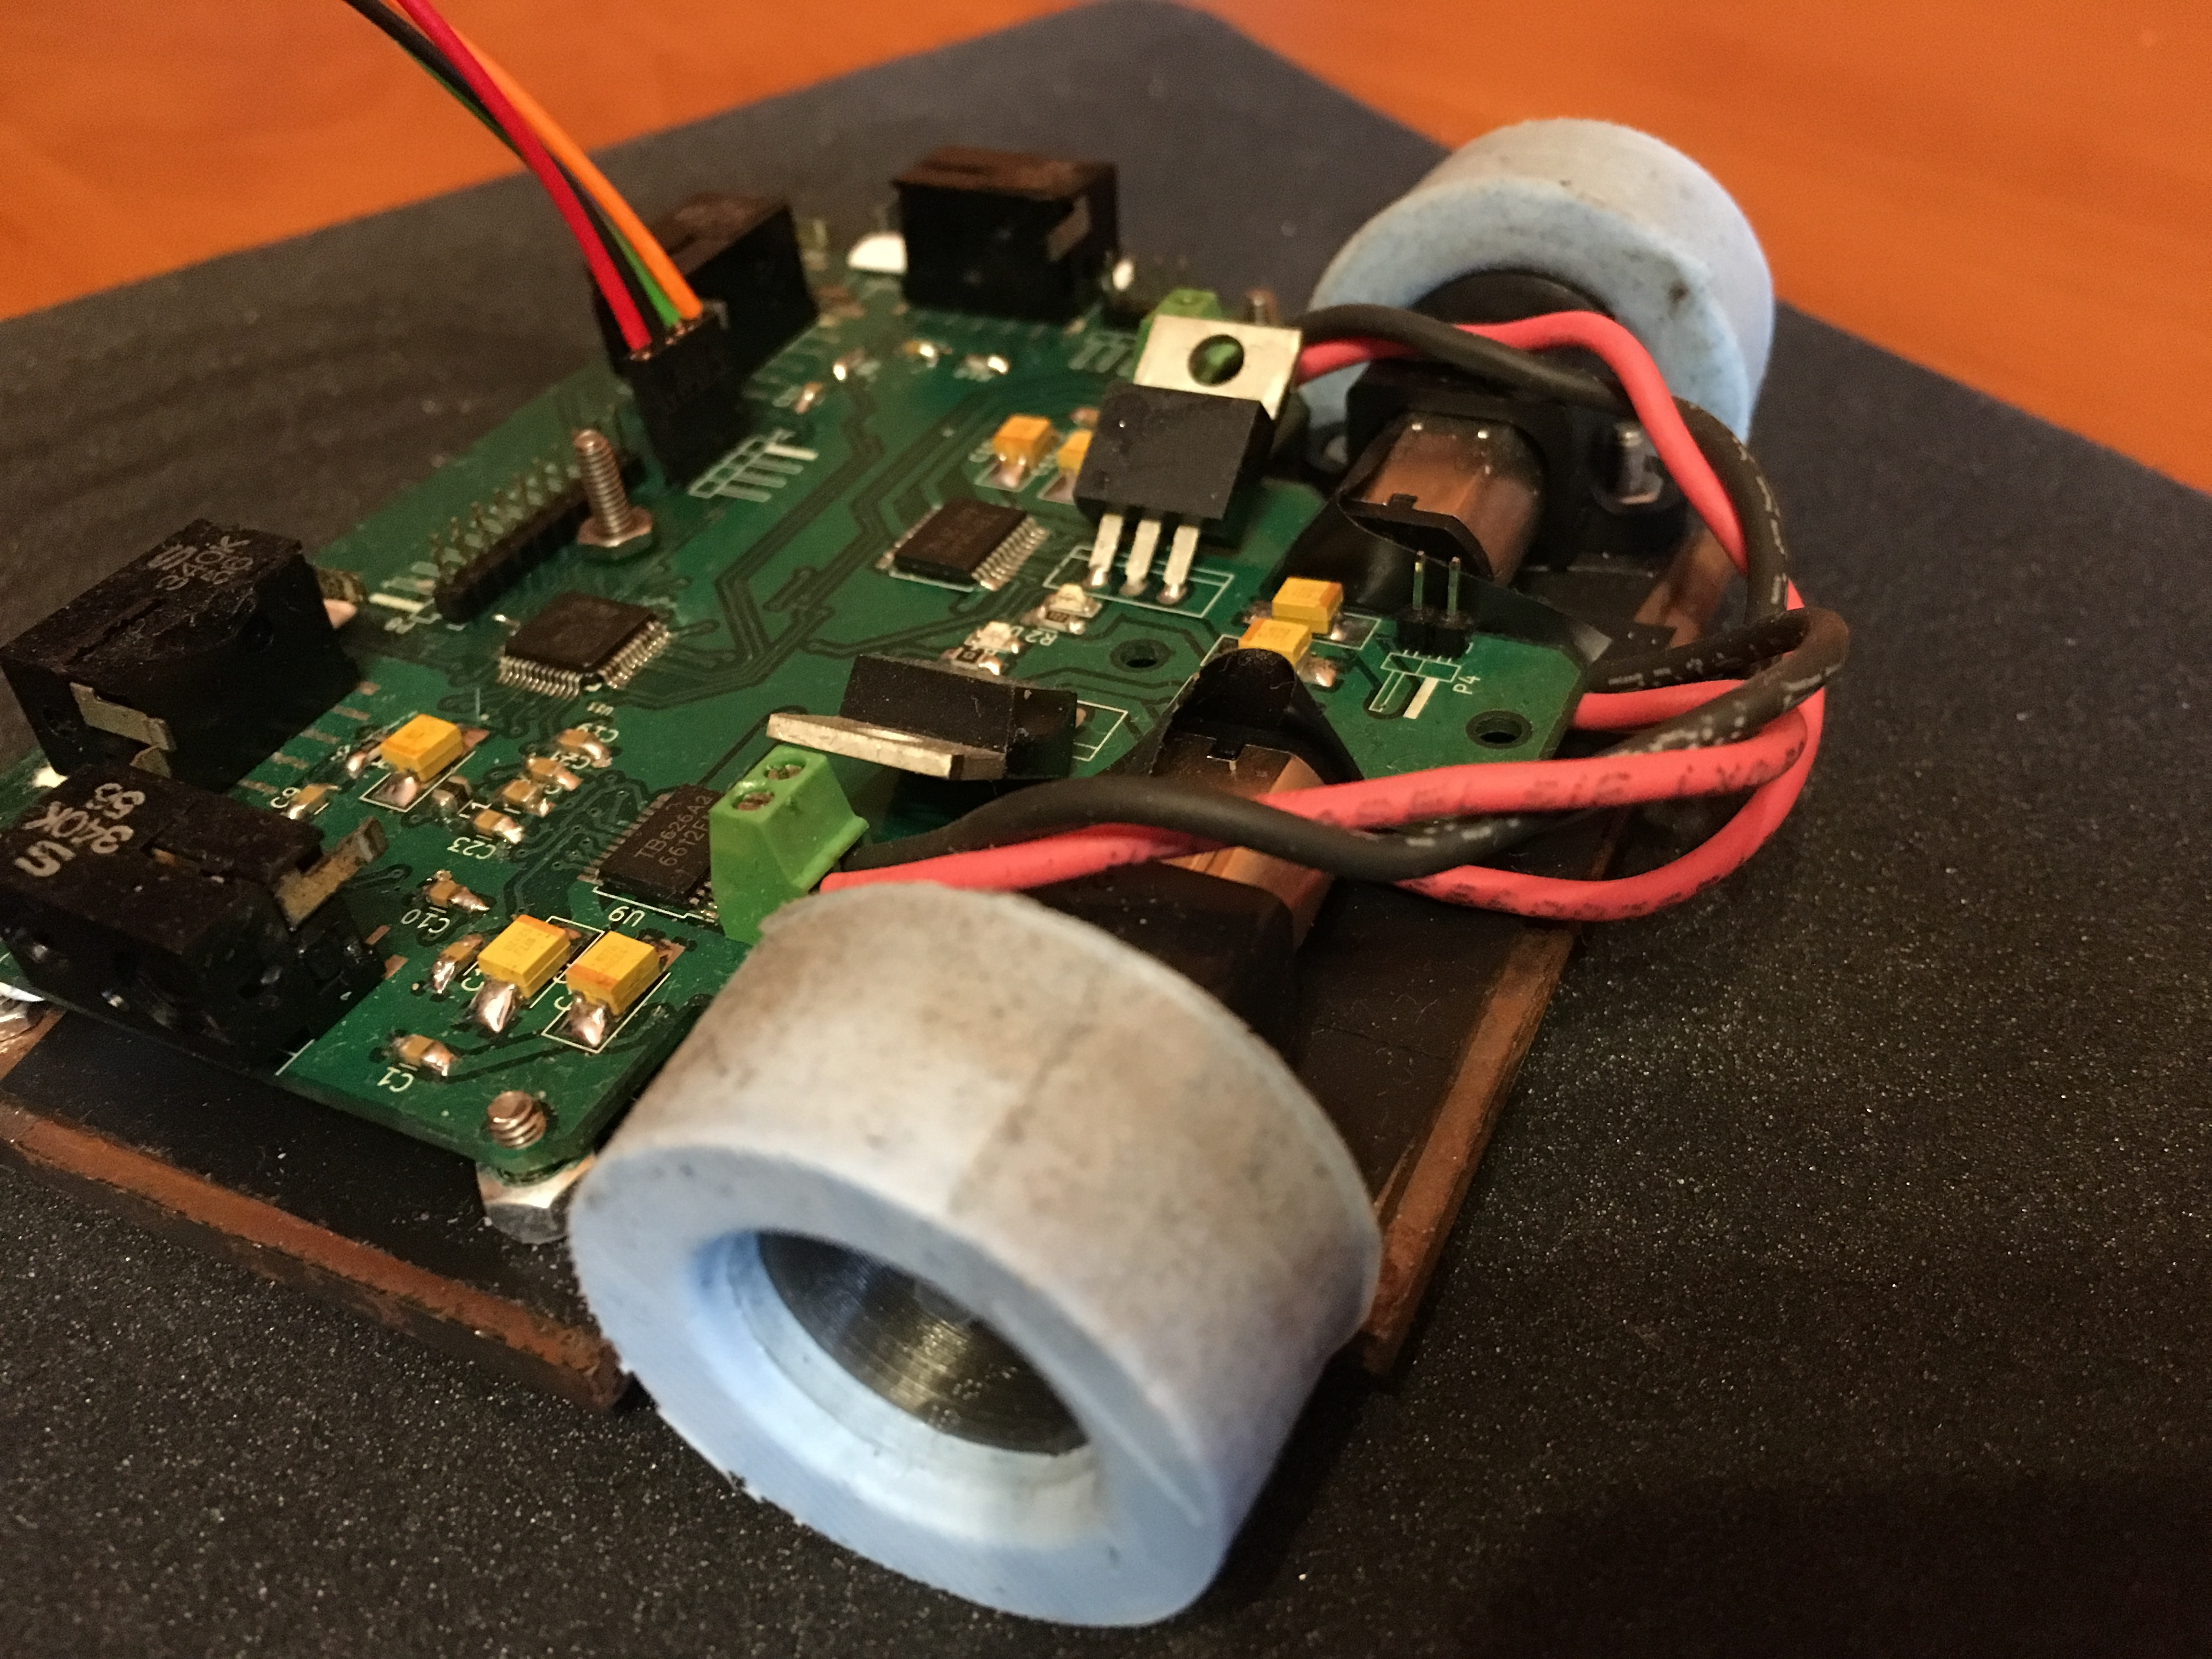
\includegraphics[width=0.75\linewidth]{pic04/drive.JPG}
	\caption{Napęd robota minisumo.}
	\label{fig:drive}	
\end{figure}

Na rysunku ~\ref{fig:drive} przedstawiono napęd robota na który składa się z dwóch silników oraz dwóch felg z oponami. Jako jednostkę napędową użyto silników \textit{Pololu HPCB} ze względu na rozmiary, dopuszczalne napięcie zasilania oraz korzystny stosunek ceny do jakości. Felgi zostały wykonane przy pomocy wydruku 3D, a opony były gotowym komponentem wykonanym z poliuretanu.

\section{Elektronika}
Projekt elektroniki robota, będącego tematem pracy dyplomowej, został stworzony przy użyciu darmowego środowiska \textit{KiCad}. Z początku płytki zostały wykonane własnoręcznie za pomocą metody termotransferu. Aczkolwiek z powodu dużej ilości przelotek, braku odpowiednich narzędzi oraz kilku błędów popełnionych na etapie projektowania, stwierdzono, iż lepszym rozwiązaniem będzie przeprojektowanie płytki oraz zlecenie wydruku firmie specjalizującej się w~tej dziedzinie. Nowa płytka była zdecydowanie trwalsza od poprzedniej wersji. Ponadto, dzięki zastosowaniu soldermaski oraz cynowania HAL, lutowanie elementów okazało się znacznie łatwiejsze.  

Docelowo robot posiada dwie płytki:
\begin{itemize}
\item główną – zawierającą całą logikę robota,
\item interfejs – pełniący rolę interfejsu użytkownika, posiadający przyciski oraz diody LED.
\end{itemize}


\begin{figure}[H]
	\centering
		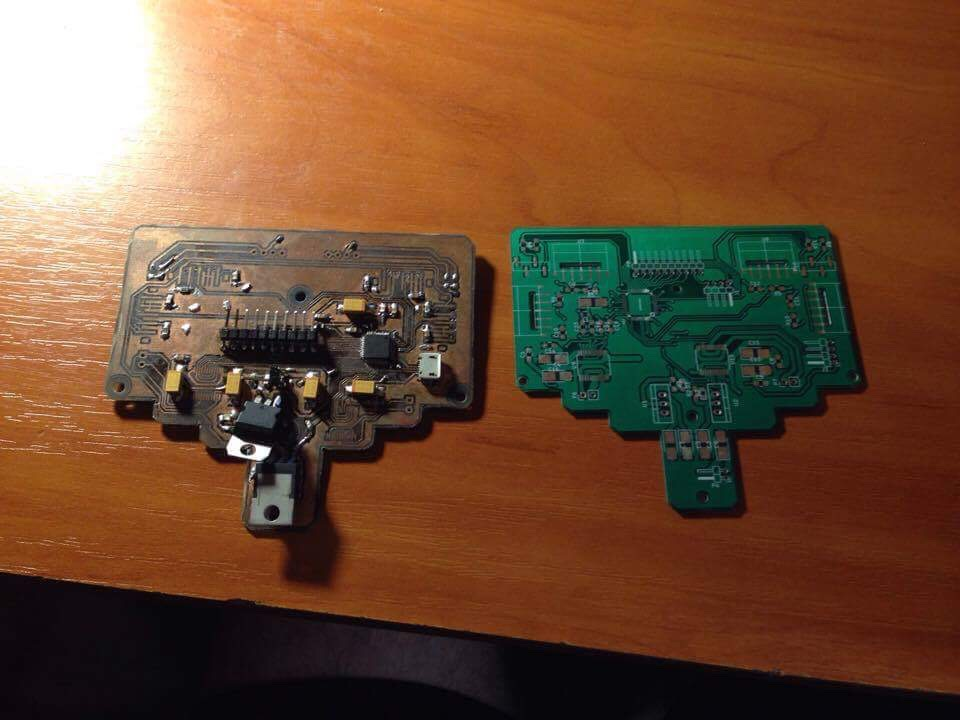
\includegraphics[width=0.75\linewidth]{pic04/boards.JPG}
	\caption{Porównanie wykonanych płytek drukowanych.}
	\label{fig:boards}	
\end{figure}

Na rysunku ~\ref{fig:boards} przedstawiono pierwszą  (wykonaną metodą termotransferu) oraz finalną (wykonaną przez firmę) wersję górnej płytki.  

\subsection{Układ zasilania}
Ze względu na ograniczone miejsce oraz dozwoloną masę za źródło zasilania posłużył akumulator litowo–polimerowy (Li–Pol) posiadający dwie cele oraz 400mAh pojemności. Bateria cechowała się wystarczającą wydajnością prądową, a pojemność pozwalała na stoczenie kilku pojedynków bez potrzeby ładowania. 

Z racji iż nie wszystkie elementy elektroniki tolerują napięcie 7.4V, układ zasilania został wyposażony w stabilizatory 3.3V oraz 5V. 

\subsection{Procesor}
Poniżej wymieniono niezbędne funkcjonalności jakie musiała spełniać docelowa jednostka obliczeniowa:

\begin{itemize}
\item przetwornik analogowo – cyfrowy (\textit{ang. ADC – analog to digital converter)} potrzebny do obsługi czujników końca ringu,
\item odpowiednia ilość portów wejścia/wyjścia dla przycisków oraz diod,
\item możliwość zmiany wypełnienia sygnału prądowego lub napięciowego (\textit{ang. Pulse–Width Modulation, PWM}) w celu odpowiedniego sterowania mocą silników,
\item interfejs UART (\textit{ang. Universal Synchronous and Asynchronous Reciever and Transmitter}) niezbędny przy komunikacji z modułem Bluetooth,
\item obsługa przerwań wykorzystywana w odbiorze wiadomości.
\end{itemize}

Powyższe wymagania spełniał procesor \textit{STM32F100C8T6B - LQFP48}. Dodatkowymi atutami była niska cena, ogólnodostępność oraz małe rozmiary.

\subsection{Sensoryka}
Konstrukcja została wyposażona w cztery czujniki \textit{SHARP Gp2y0d340k} wykrywające obecność przeciwnika do 40 centymetrów. Umieszczono je z przodu robota – dwa po bokach oraz dwa od frontu. Dodatkowo przy pługu znajdują się dwa czujniki sygnalizujące opuszczenie pola walki.

\subsection{Sterownik silników}
Jako sterownik posłużył dwukanałowy, 1.2 amperowy mostek H \textit{TB6612}. Wybór został podyktowany dostępnością oraz ceną. Aczkolwiek z czasem okazało się, iż omawiany układ jest bardzo awaryjny, a w szczególności nie nadaje się do walki w zwarciu \cite{AVR}.

\subsection{Schemat elektroniki}
W celu zwiększenia czytelności schemat podzielono na moduły, które podpisano oraz obramowano niebieską linią. 

Poniżej na zdjęciu ~\ref{fig:electric_scheme} przedstawiono schemat zaprojektowanej elektroniki (zarówno płytki górnej, jak i interfejsu).
\begin{landscape}
\begin{figure}[ht]
	\centering
		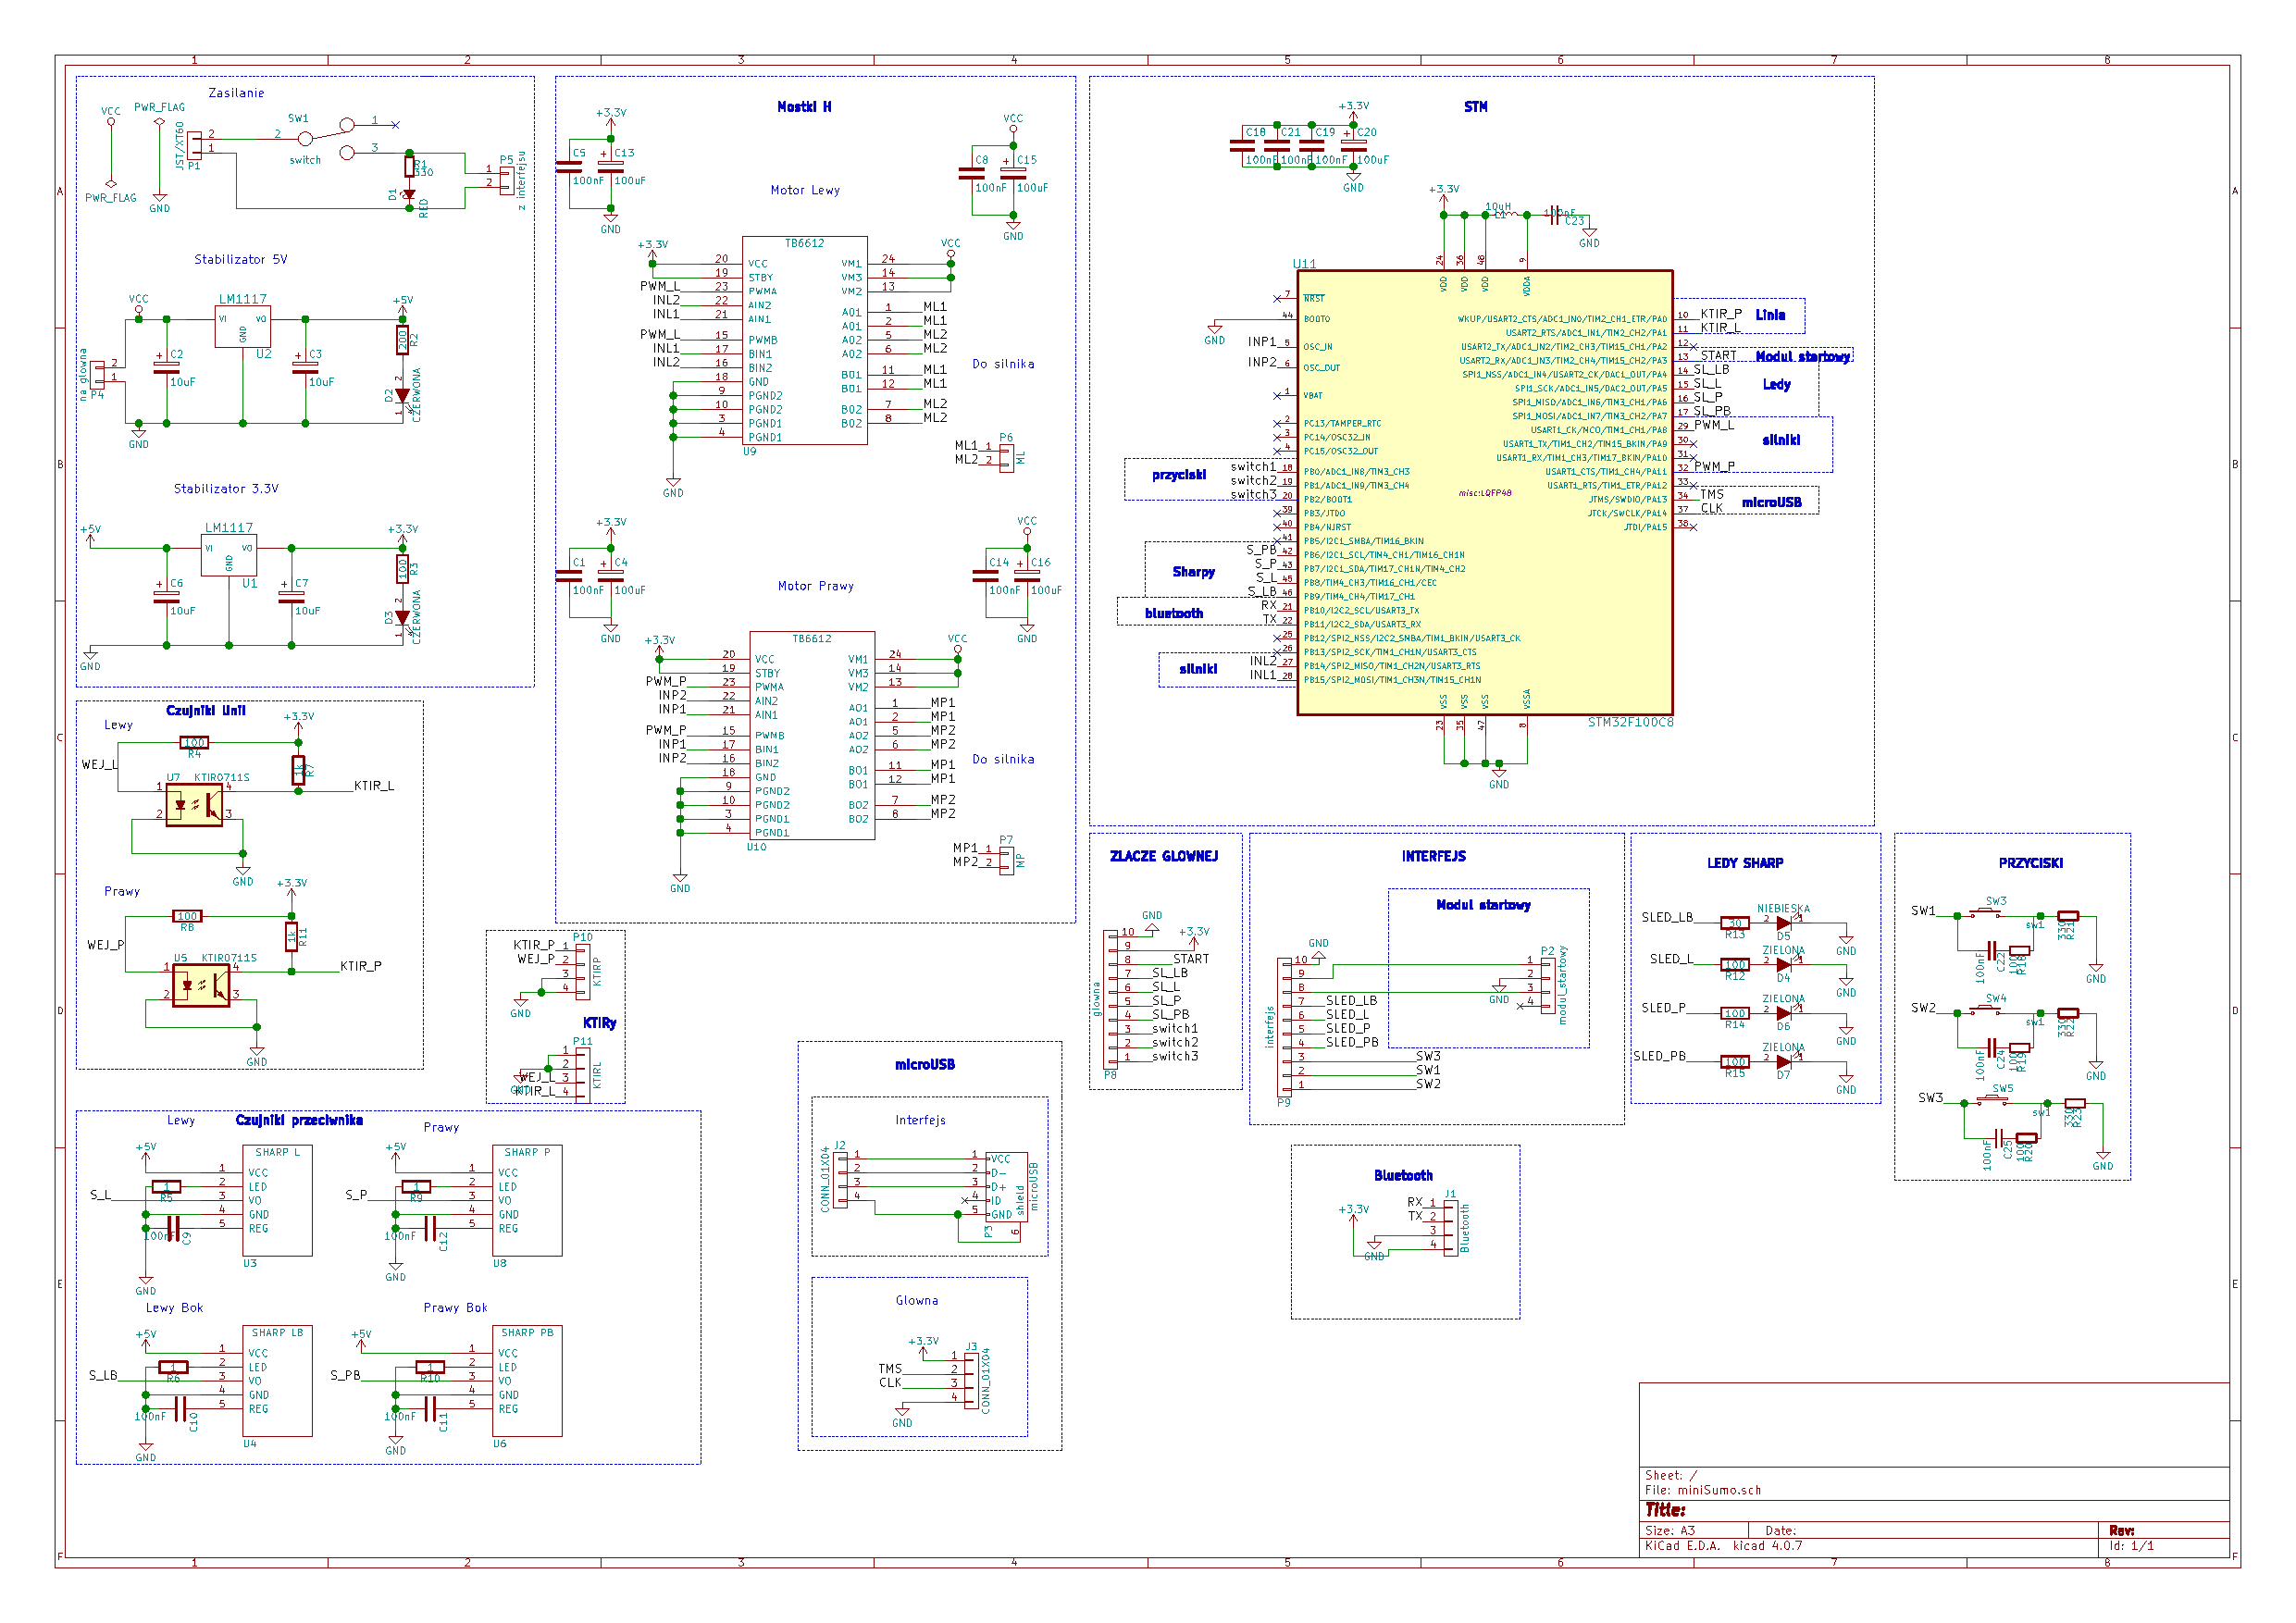
\includegraphics[width=0.8\linewidth]{pic04/electricscheme.pdf}
	\caption{Schemat elektroniki.}
	\label{fig:electric_scheme}	
\end{figure}
\end{landscape}

\section{Oprogramowanie}
Oprogramowanie sterujące robotem zostało napisane przy użyciu środowiska \textit{Eclipse}. Zawiera obsługę przychodzących/nadawanych wiadomości, zarządza sensoryką oraz motoryką konstrukcji. 

\subsection{Transmisja danych}
Transmisja danych opiera się na przesyłaniu ciągu liczb tak jak to opisano w 3. rozdziale. Przechwytywanie wiadomości odbywa się przy użyciu przerwania, które zostaje obsłużone w momencie zmiany stanu logicznego na pinie RX (połączonego z modułem Bluetooth) procesora. Następnie zostaje wywołana funkcja obsługująca przerwanie, przerywając tym samym aktualnie wykonywany kod. 

Listing \ref{interruptcode} przedstawia funkcję wywoływaną w momencie przerwania. Pierwszą czynnością było zapisanie odebranej wiadomości do zmiennej tablicowej \textit{received\_message}. Linia 6 przedstawia przypisanie pierwszej liczby otrzymanej wiadomości do zmiennej \textit{option}, która kolejno wykorzystywana jest w warunku \textit{switch}. W zależności od jej wartości ustawiane są odpowiednie flagi, będące zmiennymi globalnymi. Po zakończeniu działania opisywanej funkcji, program zostaje wznowiony w miejscu w którym został przerwany. 

Działanie głównej funkcji programu \textit{main()} wykorzystuje pętle, które przy każdej iteracji sprawdzają stan wyżej wspomnianych flag. Na ich podstawie określana jest obecnie wykonywana funkcjonalność robota. Reszta wiadomości parsowana jest przy użyciu metody \textit{parseValueFromMessage}, a następnie interpretowana w odpowiedni sposób, zależny od obecnie wykonywanej funkcjonalności.

\begin{minipage}{\textwidth}
	\begin{lstlisting}[label=interruptcode,caption=Funkcja obsługująca przerwanie.]
void HAL_UART_RxCpltCallback(UART_HandleTypeDef *huart) {

	sscanf((char*)receive_buffer, "%s", received_message);
	HAL_GPIO_TogglePin(GPIOA, led_bt_Pin);
	char option[1];
	option[0] = received_message[0];

	switch(atoi(option)) {
	case 1:
		automatic = true;
		HAL_UART_Receive_IT(&huart3, receive_buffer, 10);
		break;
	case 2:
		debug_motors = true;
		break;
	case 3:
		debug_tires = true;
		HAL_UART_Receive_IT(&huart3, receive_buffer, 10);
		break;
	case 4:
		debug_sensors = true;
		break;
	case 5:
		remote_joystick = true;
		break;
	case 6:
		remote_gyro = true;
		break;
	default:
		debug_tires = false;
		automatic = false;
		TIM1->CCR1 = 0;
		TIM1->CCR4 = 0;
		HAL_UART_Receive_IT(&huart3, receive_buffer, 10);
	    break;
	}
}
	\end{lstlisting}
\end{minipage}
 
\subsection{Sterowanie silnikami}
Sterowanie mocą silników odbywa się za pomocą modyfikacji wypełnienia sygnału przesyłanego do sterowników silników. Zakres wartości mieści się w przedziale 0 – 100 i określa procentowy czas trwania stanu wysokiego impulsu w pojedyncznym cyklu generowanym przez \textit{timer}. 

Poniższy listing \ref{pwmcode} przedstawia fragment programu, który modyfikuje moc silników. \textit{TIM1} oznacza \textit{timer} generujący impuls, a \textit{CCR1} oraz \textit{CCR4} określają kanały, czyli docelowo silniki, do których zostanie przesłany impuls.  Wartość wypełnienia zwracana jest przez metodę \textit{parseValueFromMessage},~która parsuje odpowiedni fragment wiadomości nadesłanej z aplikacji mobilnej. 

\begin{minipage}{\textwidth}
	\begin{lstlisting}[label=pwmcode,caption=Sterowanie mocą silników.]
TIM1->CCR1 = parseValueFromMessage(3,4);
TIM1->CCR4 = parseValueFromMessage(5,6);
	\end{lstlisting}
\end{minipage}

\subsection{Obsługa czujników}
Obsługa stanu czujników została zrealizowana w bardzo prosty sposób wynikający z charakterystyki pracy sensorów. W przypadku czujników wykrywających przeciwnika sprawdzany jest stan pinu procesora, do którego podłączono wyjście sensoru. Sam czujnik działa na zasadzie diody podczerwonej generującej sygnał, który zostaje odbity od przeciwnika i trafia do odbiornika. Wyjściem czujnika jest stan wysoki w przypadku braku przeciwnika lub niski, gdy go wykryto.

\begin{minipage}{\textwidth}
	\begin{lstlisting}[label=sharpcode,caption=Obsługa czujników przeciwnika.]
if(!HAL_GPIO_ReadPin(GPIOB, sharp_l_Pin))
	transmit_message[0] = 1;

if(!HAL_GPIO_ReadPin(GPIOB, sharp_ul_Pin))
	transmit_message[1] = 1;

if(!HAL_GPIO_ReadPin(GPIOB, sharp_ur_Pin))
	transmit_message[2] = 1;

if(!HAL_GPIO_ReadPin(GPIOB, sharp_r_Pin))
	transmit_message[3] = 1;
	\end{lstlisting}
\end{minipage}

Na listingu \ref{sharpcode} przedstawiano zmianę wartości odpowiednich pól wiadomości w zależności od stanu wyjścia czujników. Wiadomość ta zostaje następnie wysłana do aplikacji mobilnej. 
\chapter{Aplikacja mobilna}
Aplikacja stworzona w ramach pracy pozwala na konfigurację oraz komunikację z wcześniej opisanym robotem minisumo. Z racji, iż została napisana w natywnym języku \textit{Swift} wspieranym systemem operacyjnym jest system iOS.

\section{Kompatybilność}
Jedynym wymogiem, który musi zostać spełniony w celu uruchomienia aplikacji jest wersja systemu – nie starsza niż \textit{iOS 10}. W związku z czym aplikacja z powodzeniem powinna działać zarówno na tabletach oraz telefonach marki \textit{Apple} posiadających wspomnianą lub nowszą wersję systemu. 

Docelowo aplikacja była uruchamiana oraz testowana na urządzeniu \textit{iPhone 5}, który jest najstarszym telefonem wspierającym system iOS 10. Powodem wyboru urządzenia była optymalizacja, a mianowicie poprawność działania aplikacji na najsłabszych podzespołach gwarantowała odpowiednią pracę na mocniejszych jednostkach.

Dodatkowo poprawność wyświetlania oraz skalowania została przetestowana w symulatorze dostarczonym wraz z środowiskiem \textit{Xcode} na urządzeniach takich jak \textit{iPhone 6 Plus} oraz \textit{iPad Pro}.
 
\section{Wzorzec MVC}
Aplikacja mobilna została zaprojektowana została według wzorca architektonicznego MVC (z~ang. \textit{Model–View–Controller}), który często wykorzystywany jest do tworzenia interfejsów użytkownika. W omawianym wzorcu można wyróżnić trzy obiekty:
\begin{itemize}
\item model – odpowiada za serwowanie danych,
\item widok – odpowiada za wizualizację danych, 
\item kontroler – reaguje na poczynania użytkownika, zarządza odświeżeniem widoków oraz aktualizacją modelu. 
\end{itemize}
Podział opisanych ról przedstawiono na rysunku ~\ref{fig:mvc}.
\begin{figure}[H]
	\centering
		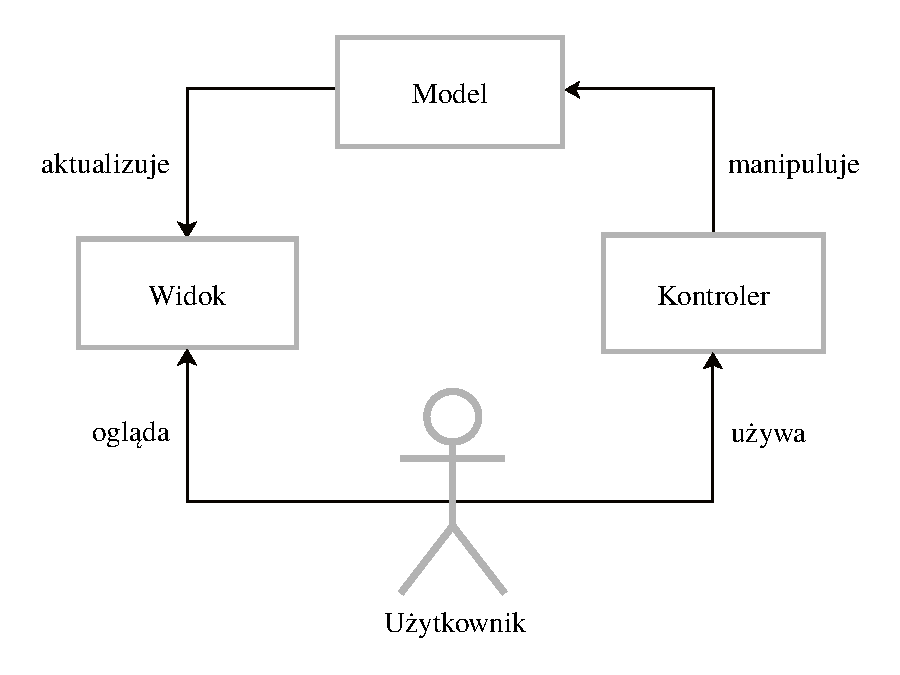
\includegraphics[width=0.75\linewidth]{pic05/mvc.pdf}
	\caption{Podział ról we wzorcu MVC.}
	\label{fig:mvc}	
\end{figure}

Dzięki wykorzystaniu tego wzorca uniezależniono przechowywane dane od sposobu w jaki są one przedstawiane użytkownikowi.

\section{Komunikacja}
Komunikacja z modułem Bluetooth została zrealizowana przy użyciu wcześniej wspomnianej platformy \textit{CoreBluetooth}. Utworzono klasę \textit{BluetoothSerial}, która była odpowiedzialna za całą logikę potrzebną do poprawnej wymiany danych między urządzeniami. Z racji, iż komunikacja jest nieodłącznym elementem każdej z funkcjonalności aplikacji skorzystano z protokołów. Protokoły są czymś na wzór intefejsów używanych w językach takich jak C++ bądź Java. Deklarują metody, lecz ich nie implementują. Każda klasa, która korzysta z komunikacji \textit{Bluetooth} musi zaimplementować metody zawarte w protokołach. Dzięki takiemu podejściu uniezależniamy logikę od kontrolerów. Klasa \textit{BluetoothSerial} nie jest w żaden sposób zależna od innych klas. Natomiast klasy, które wykorzystują komunikację, implementują odpowiednie metody w~zależności od indywidualnych konkretnych potrzeb.

\begin{minipage}{\textwidth}
	\begin{lstlisting}[label=protocolcode,caption=Protokół odpowiedzialny za komunikację między urządzeniami.]
protocol BluetoothSerialDelegate {
  func serialDidChangeState()
  func serialDidDisconnect(_ peripheral: CBPeripheral, error: NSError?)
  func serialDidReceiveString(_ message: String)
  func serialDidReadRSSI(_ rssi: NSNumber)
  func serialDidDiscoverPeripheral(_ peripheral: CBPeripheral, RSSI: NSNumber?)
  func serialDidConnect(_ peripheral: CBPeripheral)
  func serialDidFailToConnect(_ peripheral: CBPeripheral, error: NSError?)
  func serialIsReady(_ peripheral: CBPeripheral)
}
	\end{lstlisting}
\end{minipage}

Listing \ref{protocolcode} przedstawia zestaw metod zawartych w protokole komunikacyjnym. Poniżej przedstawiono przypadki w których zostają wywołane:

\begin{itemize}
\item \textit{serialDidChangeState} –  zmiana stanu modułu \textit{Bluetooth} (zostanie wyłączony lub włączony),
\item \textit{serialDidDisconnect} –  brak połączenia z modułem komunikacyjnym,
\item \textit{serialDidReceiveString} – została odebrana wiadomość typu tekstowego \textit{String},
\item \textit{serialDidReadRSSI} – gdy otrzymano sygnał RSSI (z ang. \textit{Received Signal Strength Indication}),
\item \textit{serialDidDiscoverPeripheral} – wykryto urządzenie podczas skanowania,
\item \textit{serialDidConnect} – połączono z urządzeniem, aczkolwiek urządzenie nie jest jeszcze gotowe na komunikację,
\item \textit{serialDidFailToConnect} – nie udało się nawiązać połączenia,
\item \textit{serialIsReady} – moduł jest gotowy na komunikację z aplikacją mobilną.
\end{itemize}

Tak jak wcześniej wspomniano, klasy korzystające z komunikacji mogą implementować dowolne z wyżej wymienionych metod w zależności od potrzeb.

\newpage

\section{Struktura aplikacji}
Tak jak wcześniej wspomniano, aplikacja została stworzona przy użyciu wzorca \textit{MVC}. Poniżej przedstawiono strukturę plików aplikacji.

\begin{figure}[H]
	\centering
		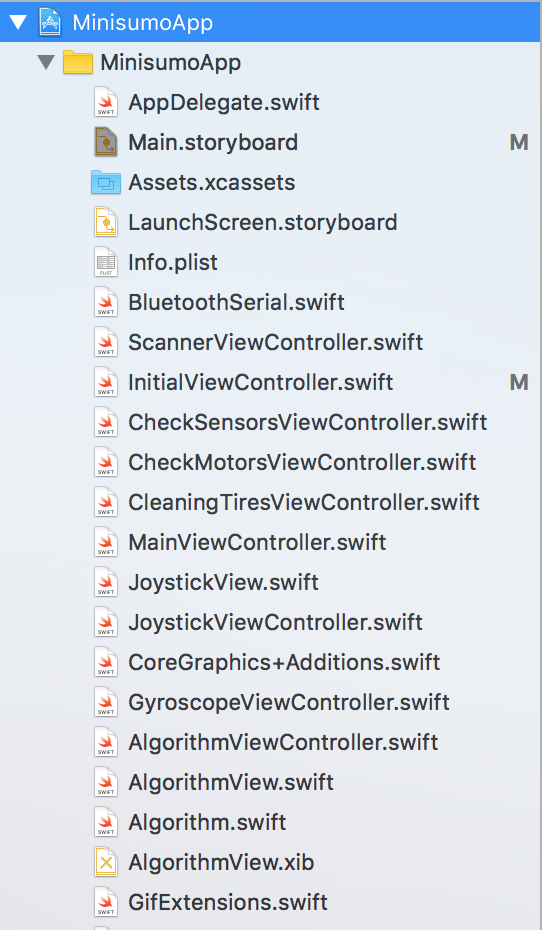
\includegraphics[width=0.75\linewidth, height=10cm, keepaspectratio]{pic05/structure.png}
	\caption{Struktura plików aplikacji mobilnej.}
	\label{fig:structure}	
\end{figure}

Na rysunku \ref{fig:structure} pliki o rozszerzeniu \textit{swift}, których nazwy kończą się na \textit{Controller} pełnią rolę kontrolerów, a \textit{View} widoków przedstawianych użytkownikowi. Reszta plików odpowiedzialna jest za logikę aplikacji. Dodatkowo plik \textit{Main.storyboard} zawiera konfiguracje większości widoków stworzonych przy użyciu graficznego narzędzia dostarczonego przez środowisko \textit{Xcode}.

\subsection{Panel powitalny}
Panel powitalny jest pierwszym widokiem z którym użytkownik ma do czynienia po uruchomieniu aplikacji mobilnej. Odpowiada on za poprawne wykrycie urządzenia \textit{Bluetooth} oraz dalszą komunikację. Składa się z elementów takich jak krótka instrukcja obsługi oraz przycisk \textit{Connect}, który po wciśnięciu wyświetla listę urządzeń gotowych na połączenie. Dodatkowo w przypadku wyłączonej komunikacji \textit{Bluetooth} zostanie wyświetlony komunikat o konieczności jej włączenia. 

\newpage

Po lewej stronie na rysunku \ref{fig:initial} przedstawiono omawiany panel, natomiast rysunek \ref{fig:scanner} po prawej stronie przedstawia listę dostępnych urządzeń.

\begin{figure}[H]
\centering
\begin{minipage}{.5\textwidth}
  \centering
  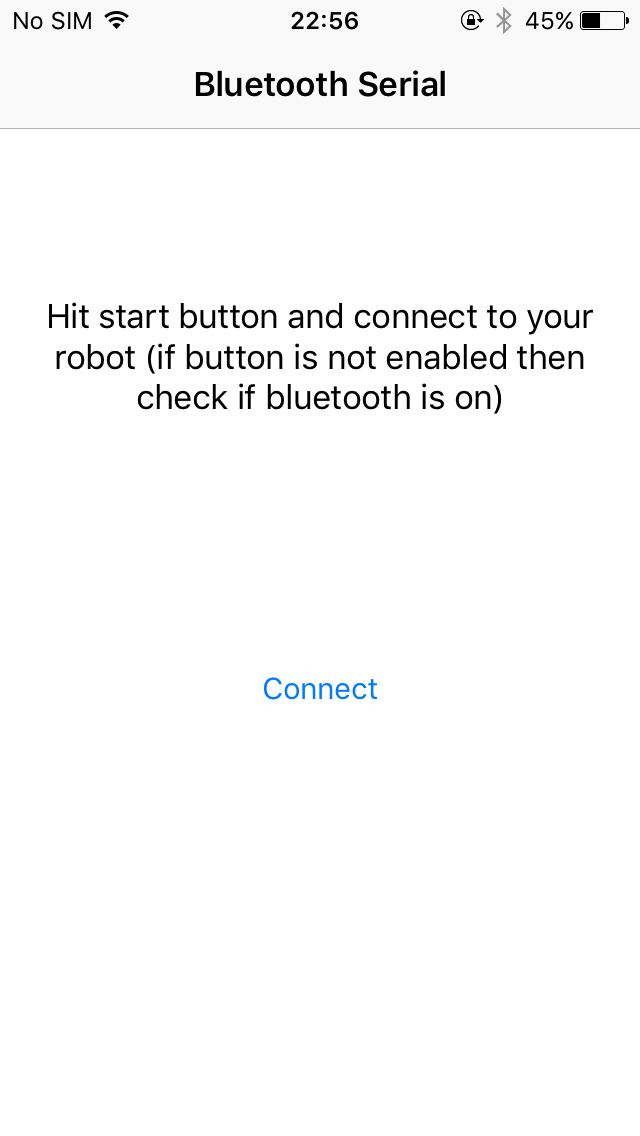
\includegraphics[width=.75\linewidth, height=10cm, keepaspectratio, fbox]{pic05/initial.PNG}
  \caption{Widok połączenia.}
  \label{fig:initial}
\end{minipage}%
\begin{minipage}{.5\textwidth}
  \centering
  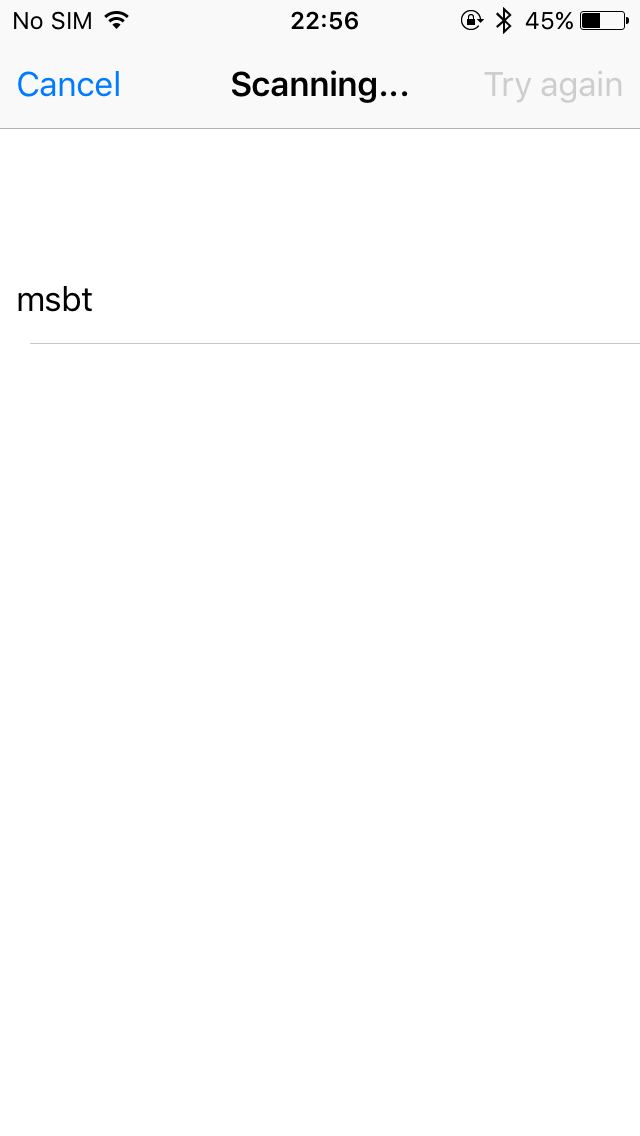
\includegraphics[width=.75\linewidth, height=10cm, keepaspectratio, fbox]{pic05/scanning.PNG}
  \caption{Widok dostępnych urządzeń.}
  \label{fig:scanner}
\end{minipage}
\end{figure}

Za obsługę panelu powitalnego odpowiedzialna jest klasa \textit{InitialViewController}, która inicjalizuje globalny obiekt \textit{serial} , wykorzystywany do komunikacji \textit{Bluetooth} w obrębie całej aplikacji. Zdecydowano się na taki krok, ponieważ transmisja danych jest nieodłącznym elementem każdej funkcjonalności aplikacji, przez co uniknięto problemu z przekazywaniem obiektu pomiędzy kontrolerami.

\begin{minipage}{\textwidth}
	\begin{lstlisting}[label=scannerprotocol,caption=Implementacja protokołu.]
func serialDidDiscoverPeripheral(_ peripheral: CBPeripheral, RSSI: NSNumber?) {
  for exisiting in peripherals {
     if exisiting.peripheral.identifier == peripheral.identifier { return }
  }
    let theRSSI = RSSI?.floatValue ?? 0.0
    peripherals.append(peripheral: peripheral, RSSI: theRSSI)
    peripherals.sort { $0.RSSI < $1.RSSI }
    tableView.reloadData()
}
  
func serialDidFailToConnect(_ peripheral: CBPeripheral, error: NSError?) {
  tryAgainButton.isEnabled = true
}
  
func serialDidDisconnect(_ peripheral: CBPeripheral, error: NSError?) {
  tryAgainButton.isEnabled = true
}
  
func serialIsReady(_ peripheral: CBPeripheral) {
  performSegue(withIdentifier: "ShowMainViewController", sender: nil)
}
  
func serialDidChangeState() {
   if serial.centralManager.state != .poweredOn {
     dismiss(animated: true, completion: nil)
   }
}
	\end{lstlisting}
\end{minipage}

Listing \ref{scannerprotocol} przedstawia implementację metod zawartych w protokole \textit{BluetoothSerialDelegate} (omówionym w rozdziale 5.3) dla klasy \textit{ScannerViewController} odpowiedzialnej za wyświetlenie wykrytych urządzeń oraz poprawne połączenie z wybranym urządzeniem. Metoda \textit{serialDidDiscoverPeripheral} agreguje wykryte urządzenia, a następnie wysyła do widoku żądanie o wyświetleniu posortowanej listy ze znalezionymi urządzeniami. Funkcje \textit{serialDidFailToConnect} oraz \textit{serialDidDisconnect} odpowiedzialne są za przypadek, gdy nie udało się ustanowić połączenia z modułem \textit{Bluetooth} – wyświetlają przycisk dzięki któremu możliwa jest ponowna próba połączenia. Gdy aplikacja mobilna poprawnie ustanowiła połączenie z którymś z urządzeń, uruchamiana jest funkcja \textit{serialIsReady}, której wynikiem jest przejście do panelu głównego.  Natomiast w przypadku rozłączenia wywoływana jest metoda \textit{serialDidChangeState}, która wywołuje powrót do poprzedniego widoku jakim jest widok powitalny.

\subsection{Panel główny}
Panel główny odpowiedzialny jest tylko i wyłącznie za nawigację do poszczególnych funkcjonalności aplikacji. Składa się z prostego kontrolera \textit{MainViewController}, który nawiguje do odpowiednich paneli w zależności od wciśniętego przycisku.

\begin{figure}[H]
	\centering
		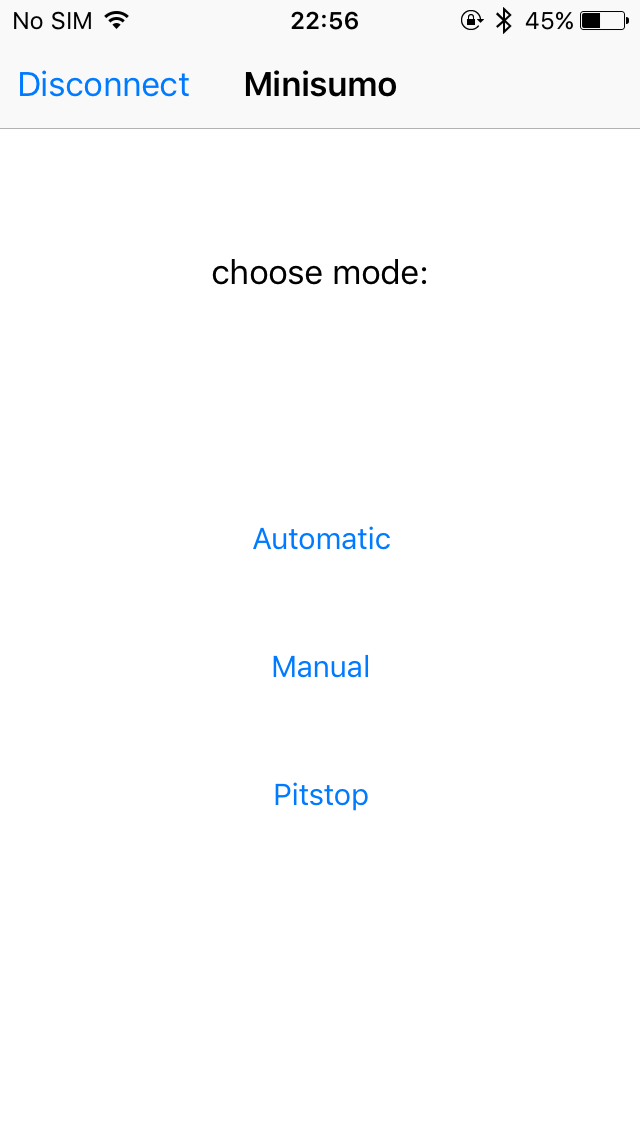
\includegraphics[width=0.75\linewidth, height=10cm, keepaspectratio, fbox]{pic05/main.PNG}
	\caption{Panel główny aplikacji mobilnej.}
	\label{fig:mainview}	
\end{figure}

Na rysunku \ref{fig:mainview} przedstawiono wygląd panelu głównego aplikacji. Można zauważyć trzy przyciski \textit{Automatic}, \textit{Manual}, \textit{Pitstop}, które nawigują odpowiednio do panelu sterowania automatycznego, zdalnego oraz diagnostyki. 

\subsection{Panel sterowania automatycznego}
Panel sterowania automatycznego został stworzony w celu testowania algorytmów walki oraz konfigurowania robota do zawodów. Zaprojektowano go tak, aby był jak najbardziej intuicyjny w użytkowaniu. W górnej części widoku umiejscowione zostało zdjęcie formatu \textit{.gif} przedstawiające zachowanie robota na ringu dla danego algorytmu. Poniżej wizualizacji znajduje się krótki opis działania strategii, okno do ustawienia maksymalnej procentowej mocy silników oraz przełącznik, który określa czy robot powinien czekać na sygnał startowy (opcja wymagana podczas większości zawodów. Jej celem jest zapewnienie równego startu walczących ze sobą robotów). Na dole znajduje się przycisk \textit{START}, który po wciśnięciu wysyła do robota wiadomość z konfiguracją. Przerwanie walki następuje po wciśnięciu przycisku \textit{STOP} (który jest widoczny po wciśnięciu przycisku \textit{START}).  W celu zmiany algorytmu należy przesunąć ekran od prawej do lewej lub na odwrót. Na samym dole znajdują się kropki odpowiadające każdemu z algorytmów, a najjaśniejsza z nich sygnalizuje, która strategia jest obecnie konfigurowana.

Rysunek \ref{fig:automaticview} ukazuje wygląd opisywanego panelu sterowania automatycznego (zamiast wizualizacji działania algorytmu walki wstawiono losowe zdjęcie). 

\begin{figure}[H]
	\centering
		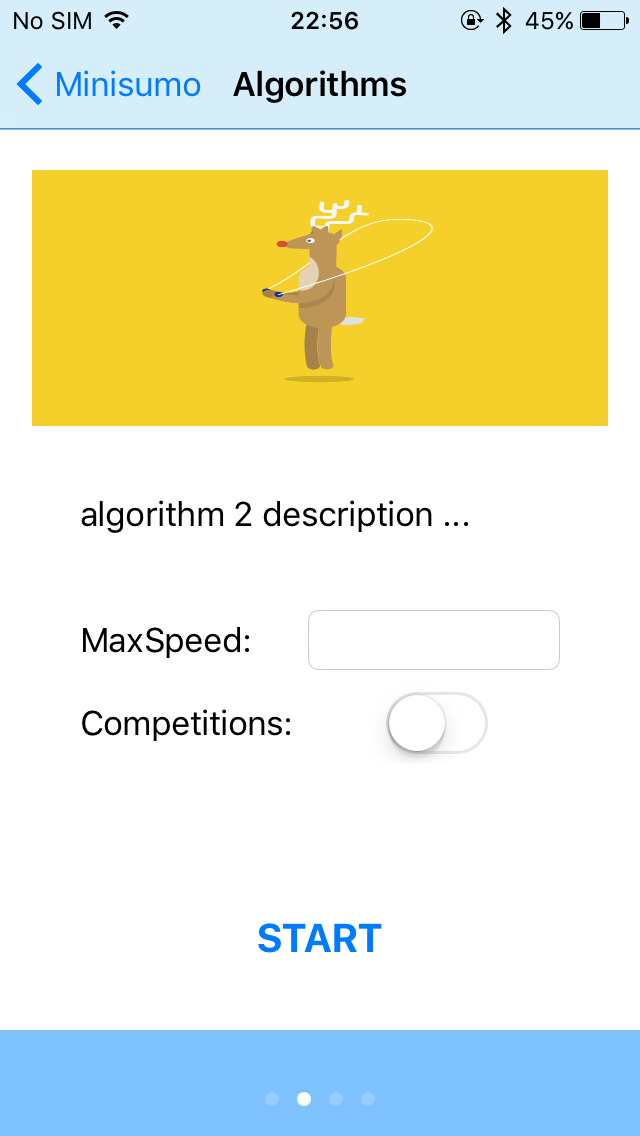
\includegraphics[width=0.75\linewidth, height=10cm, keepaspectratio, fbox]{pic05/algorithm.PNG}
	\caption{Panel sterowania automatycznego aplikacji mobilnej.}
	\label{fig:automaticview}	
\end{figure}

Za obsługę panelu sterowania automatycznego  odpowiada klasa 	\textit{AlgorithmViewController}, która wszystkie algorytmy walki przechowuje w tablicy \textit{algorithms} w postaci obiektów klasy \textit{Algorithm}.
  
\begin{minipage}{\textwidth}
	\begin{lstlisting}[label=algorithmclass,caption=Klasa Algorithm.]
class Algorithm {
  var description = ""
  var videoName = ""
  var isCompetition = false
}
	\end{lstlisting}
\end{minipage}

Listing \ref{algorithmclass} przedstawia klasę \textit{Algorithm}, która zawiera pola typu tekstowego \textit{description}, \textit{videoName} oraz logicznego \textit{isCompetition} odpowiadające odpowiednio opisowi działania algorytmu walki, ścieżce zdjęcia \textit{.gif} obrazującego zachowanie robota oraz informacji odnośnie tego czy robot powinien oczekiwać na sygnał startowy.
 
\subsection{Panel sterowania zdalnego}
Panel sterowania zdalnego pozwala na zdalne sterowanie silnikami robota za pomocą akcelerometru bądź wirtualnego dżojstiku. Podobnie jak panel główny, posiada  widok z dwoma przyciskami, które nawigują do poszczególnych funkcjonalności:
 
\subsubsection{Sterowanie akcelerometrem}
Sterowanie akcelerometrem pozwala na zdalne sterowaniem ruchem robota poprzez odpowiednie przechylenie telefonem. Sam panel składa się z krótkiej instrukcji obsługi, informacji o mocy oraz kierunku jazdy oraz przycisku \textit{START}, który służy do uruchomienia omawianej funkcjonalności.


Rysunek \ref{fig:accview} przedstawia wygląd omawianego panelu. Warto zauważyć, iż dla wygody został on zaprojektowany w orientacji poziomej.

\begin{figure}[H]
	\centering
		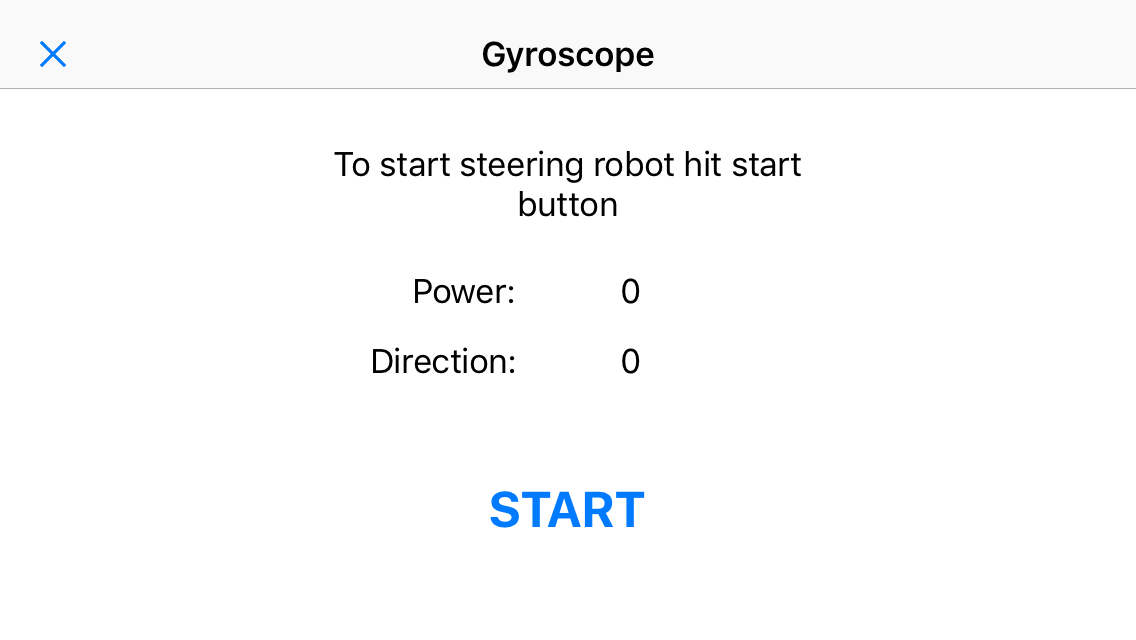
\includegraphics[width=0.75\linewidth, height=10cm, keepaspectratio, fbox]{pic05/gyro.PNG}
	\caption{Panel sterowania zdalnego akcelerometrem.}
	\label{fig:accview}	
\end{figure}

W celu realizacji wyżej wspomnianej funkcjonalności wykorzystano obrót urządzenia wokół osi Y oraz Z. Obrót wokół osi Y odzwierciedla ruch robota w przód oraz w tył, natomiast obrót wokół osi Z kierunek ruchu – lewo lub prawo. Im większe wychylenie tym większa prędkość lub mocniejszy skręt. Dla lepszego zobrazowania problemu na rysunku \ref{fig:axis} przedstawiono orientację urządzenia.

\begin{figure}[H]
	\centering
		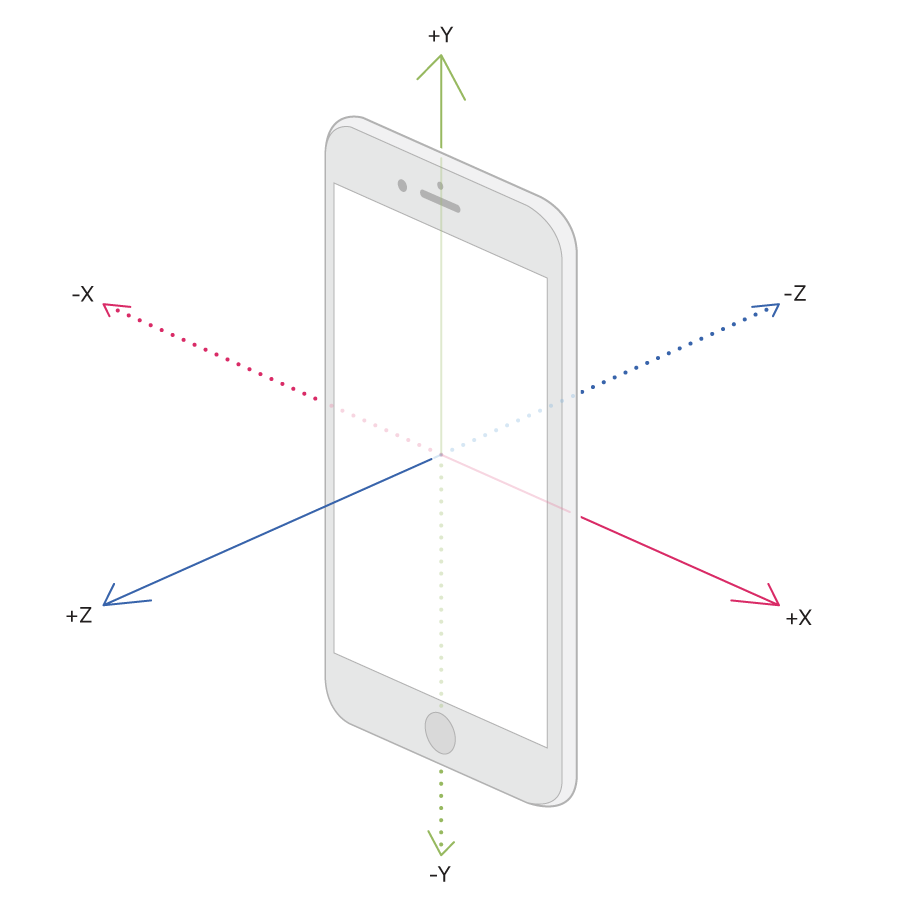
\includegraphics[width=0.6\linewidth]{pic05/axis}
	\caption{Osie X, Y oraz Z określające orientację urządzenia \cite{Axis}.}
	\label{fig:axis}	
\end{figure}

Listing \ref{accfunc} przedstawia fragment kodu, należący do klasy \textit{GyroscopeViewController}, a dokładniej metodę \textit{startAcc}, która zostaje wywołana w momencie wciśnięcia przycisku \textit{START}. Linia 2 ustawia czas, co który będzie zczytywany pomiar wychylenia urządzenia (w tym przypadku pomiar dokonywany jest co 200 milisekund). Następne zostaje uruchomiony akcelerometr oraz przechwytywane są wartości obrotów wokół wspomnianych wcześniej osi. Ich wartości zawierają się w zakresie od -1 do 1. Na ich podstawie określane są kierunek oraz prędkość, które zostaną wysłane do robota.

\begin{minipage}{\textwidth}
	\begin{lstlisting}[label=accfunc,caption=Implementacja metody startAcc.]
func startAcc() {
  motionManager.deviceMotionUpdateInterval = 0.2
  motionManager.startDeviceMotionUpdates(to: OperationQueue.current!) { (data, error) in
  if let motion = data {
    var turn = Int(100 * motion.attitude.pitch)
    var power = Int(100 * motion.attitude.roll)
    
    . . . 

  }
   . . . 
}
	\end{lstlisting}
\end{minipage}

\subsubsection{Sterowanie wirtualnym dżojstikiem}
Sterowanie odbywa się za pomocą dwuwymiarowego drążka w postaci niebieskiego koła. Wychylenie drążka wpływa na kierunek jazdy oraz prędkość kół konstrukcji (im większe wychylenie tym większa prędkość). Dzięki zastosowaniu takiego rozwiązania możliwa jest jazda w przód oraz w tył. Dodatkowo w górnej części widoku znajduje się informacja odnośnie kierunku jazdy, wyrażonej kątowo w stopniach oraz mocy silników wyrażonej procentowo. Warto dodać, iż po puszczeniu drążka wraca on do początkowego położenia, które jest jednoznaczne z brakiem ruchu robota.

\begin{figure}[H]
	\centering
		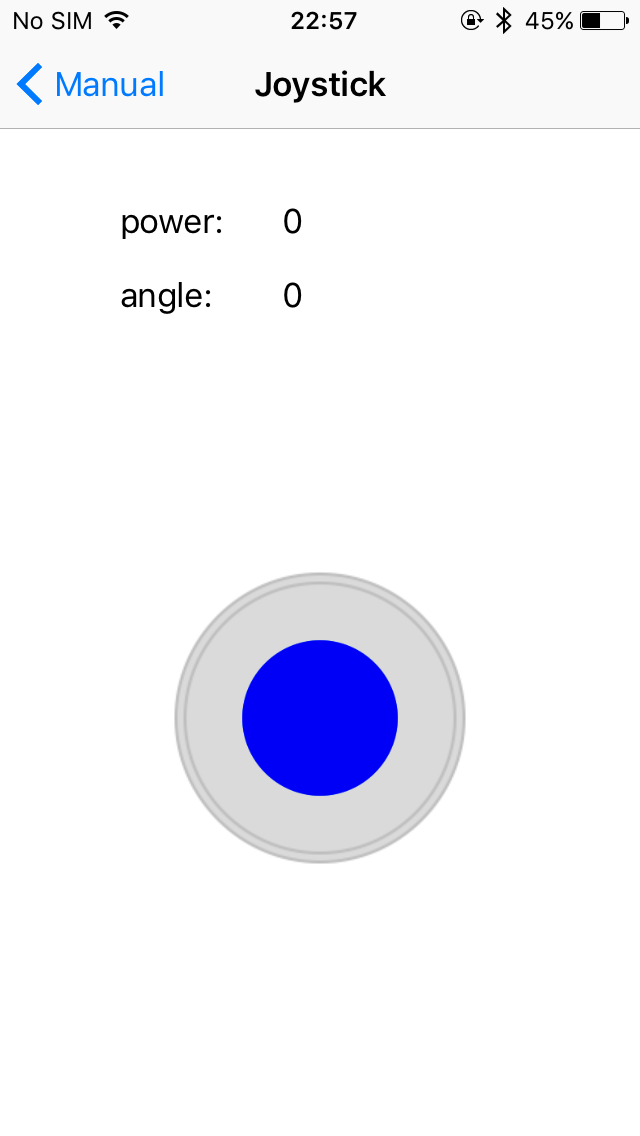
\includegraphics[width=0.75\linewidth, height=10cm, keepaspectratio, fbox]{pic05/joystick.PNG}
	\caption{Panel sterowania zdalnego dżojstikiem.}
	\label{fig:joystickview}	
\end{figure}

Powyższy rysunek \ref{fig:joystickview} przedstawia wygląd panelu służącego do zdalnego sterowania robotem za pomocą dżojstiku.

\begin{figure}[H]
	\centering
		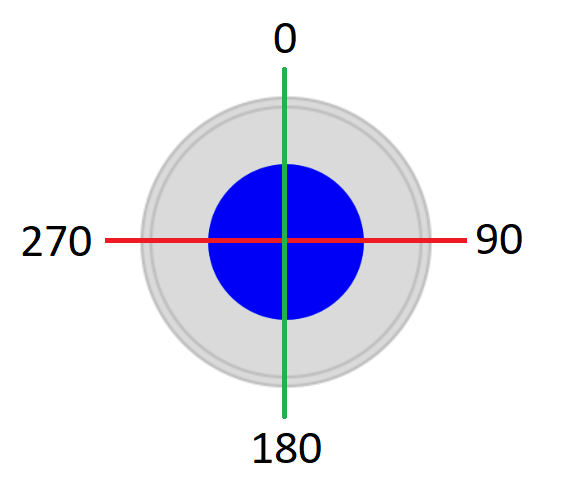
\includegraphics[width=0.75\linewidth]{pic05/joy.png}
	\caption{Wirtualny dżojstik.}
	\label{fig:joystickdirections}	
\end{figure}

Rysunek \ref{fig:joystickdirections} przedstawia zależność kierunku jazdy konstrukcji od kąta odchylenia drążka. Jak łatwo zauważyć, górna półkula odpowiedzialna jest za jazdę w przód, natomiast dolna w~tył (półkule zostały oddzielone czerwoną kreską). Analogicznie lewa półkula pozwala na jazdę w~lewo, a prawa w prawo (półkule zostały oddzielone zieloną kreską). Dodatkowo w celu ułatwienia oszacowania żądanej mocy silników utworzono szary okrąg, który wyznacza granicę maksymalnego wychylenia drążka.

Za zdalne sterowanie wirtualnym dżojstikiem odpowiedzialna jest klasa \textit{JoystickView}, (implementuje wygląd oraz położenie drążka) oraz klasa  \textit{JoystickViewController}, która nasłuchuje zmian położenia drążka oraz wysyła odpowiednią informację do robota. 

\begin{minipage}{\textwidth}
	\begin{lstlisting}[label=joystickcontrol,caption=Metoda klasy JoystickViewController.]
override func viewWillAppear(_ animated: Bool) {
    
   super.viewWillAppear(animated)
   serial.delegate = self
   msg[0] = "5"
   let rect = view.frame
   let size = CGSize(width: 150.0, height: 150.0)
   let joystick1Frame = CGRect(origin: CGPoint(x: rect.width/2 - size.width/2, y: rect.height/2), size: size)
   let joystick1 = JoyStickView(frame: joystick1Frame)
    
   view.addSubview(joystick1)
   joystick1.movable = false
   joystick1.alpha = 1.0
   joystick1.baseAlpha = 0.5 
   joystick1.handleTintColor = UIColor.blue
    
   joystick1.monitor = { angle, displacement in
     let power = Int(100 * displacement)
     let direction = Int(angle)

     self.leftTheta.text = "\(direction)"
     self.leftMagnitude.text = "\(power) %"
	
	 . . .
	
     usleep(useconds_t(20 * self.ms))
     serial.sendMessageToDevice(self.msg.joined())
   }
}  
	\end{lstlisting}
\end{minipage}

Powyższy listing \ref{joystickcontrol} przedstawia implementajcę najważniejszej funkcji klasy \textit{JoystickViewController}, którą jest \textit{viewWillAppear}. Jest to funkcja dostarczona przez platformę \textit{UIViewController} automatycznie wywoływana po załadowaniu widoku. Linia 5 przedstawia ustawienie pierwszego znaku wiadomości, która informuje robota jaka funkcjonalność powinna zostać obsłużona. Linie 6 – 15 ukazują konfigurację wyglądu dżojstiku, natomiast linia 17 deklaruje nasłuchiwanie zmian położenia drążka, które zwraca zmienne typu \textit{float}: \textit{angle} oraz \textit{displacement}, określające kąt (zakres 0 – 360 stopni) oraz wysunięcie (wartość od 0 do 1) drążka. Linia 18 skaluje wartość wysunięcia tak, aby wartość mieściła się w przedziale 0 – 100, co jest podyktowane wymogiem struktury wysyłanej wiadomości. Następnie w liniach 21 – 22 aktualizowane są informacje dostarczane użytkownikowi. Po odpowiednim przeliczeniu otrzymanych wartości na kierunki oraz moce silników następuje wysłanie wiadomości do robota (linia 27) poprzedzone 20 milisekundowym opóźnieniem (linia 26). Zastosowane opóźnienie spowodowane było ograniczoną przepustowością modułu \textit{Bluetooth} oraz niską wydajnością aplikacji. Dzięki opóźnieniu uzyskano pewność obsługi każdej wysłanej wiadomości kosztem niezauważalnego opóźnienia aktualizacji widoku przesunięcia drążka.

\subsection{Panel diagnostyki}
Panel diagnostyki powstał z myślą o sprawdzeniu poprawności działania poszczególnych komponentów robota. Niejednokrotnie zdarzało się, iż robot zachowywał się w nieoczekiwany sposób. Wtedy pojawiało się pytanie, czy wina leży po stronie oprogramowania, czy któryś z komponentów nie działa prawidłowo. Dzięki panelowi diagnostyki uzyskano możliwość szybszego zdiagnozowania problemu. 
Stworzony widok składa się z trzech zakładek:\textit{Sensors, Motors} oraz \textit{Tires} . Nawigowanie między funkcjonalnościami odbywa się za pomocą kliknięcia jednej z zakładek widocznych u dołu ekranu. 

\begin{figure}[H]
	\centering
		
\includegraphics[width=0.75\linewidth, fbox]{pic05/tabs}
	\caption{Widok zakładek w panelu diagnostyki.}
	\label{fig:pitstopview}	
\end{figure}

Rysunek \ref{fig:pitstopview} przedstawia zakładki nawigujące do poszczególnych opcji diagnostycznych.

\newpage

\subsubsection{Diagnostyka czujników}
Panel diagnostyki czujników powstał z myślą o sprawdzeniu poprawności działania czterech czujników wykrywających przeciwnika. Po włączeniu tego widoku zostaje wysłana wiadomość do robota z żądaniem obsłużenia odpowiedniej funkcjonalności. Następnie co 20 milisekund robot wysyła informację zwrotną, zawierającą stan czujników. W przypadku, gdy któryś z czujników wykrył obiekt znajdujący się przed nim, na ekranie pojawia się etykieta \textit{work} w odpowiednim miejscu. Klasą odpowiedzialną za obsługę funkcjonalności jest \textit{CheckSensorsViewController}.

\begin{figure}[H]
	\centering
		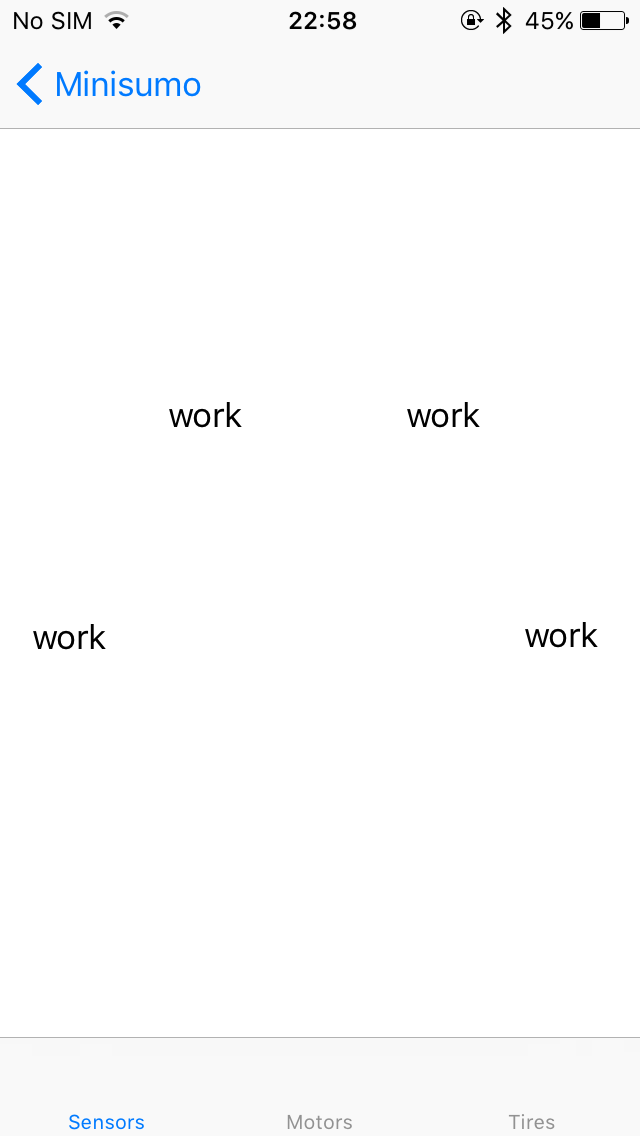
\includegraphics[width=0.75\linewidth, height=10cm, keepaspectratio, fbox]{pic05/sensors.PNG}
	\caption{Widok diagnostyki czujników.}
	\label{fig:diagsensors}	
\end{figure}

Rysunek \ref{fig:diagsensors} ukazuje widok diagnostyki czujników. Przedstawiono na nim przypadek, gdzie każdy z czujników wykrył przeciwnika. Górne etykiety odpowiadają czujnikom znajdującym się w frontalnej części robota, natomiast boczne odpowiadają odpowiednio lewemu oraz prawemu czujnikowi.


\begin{figure}[H]
	\centering
		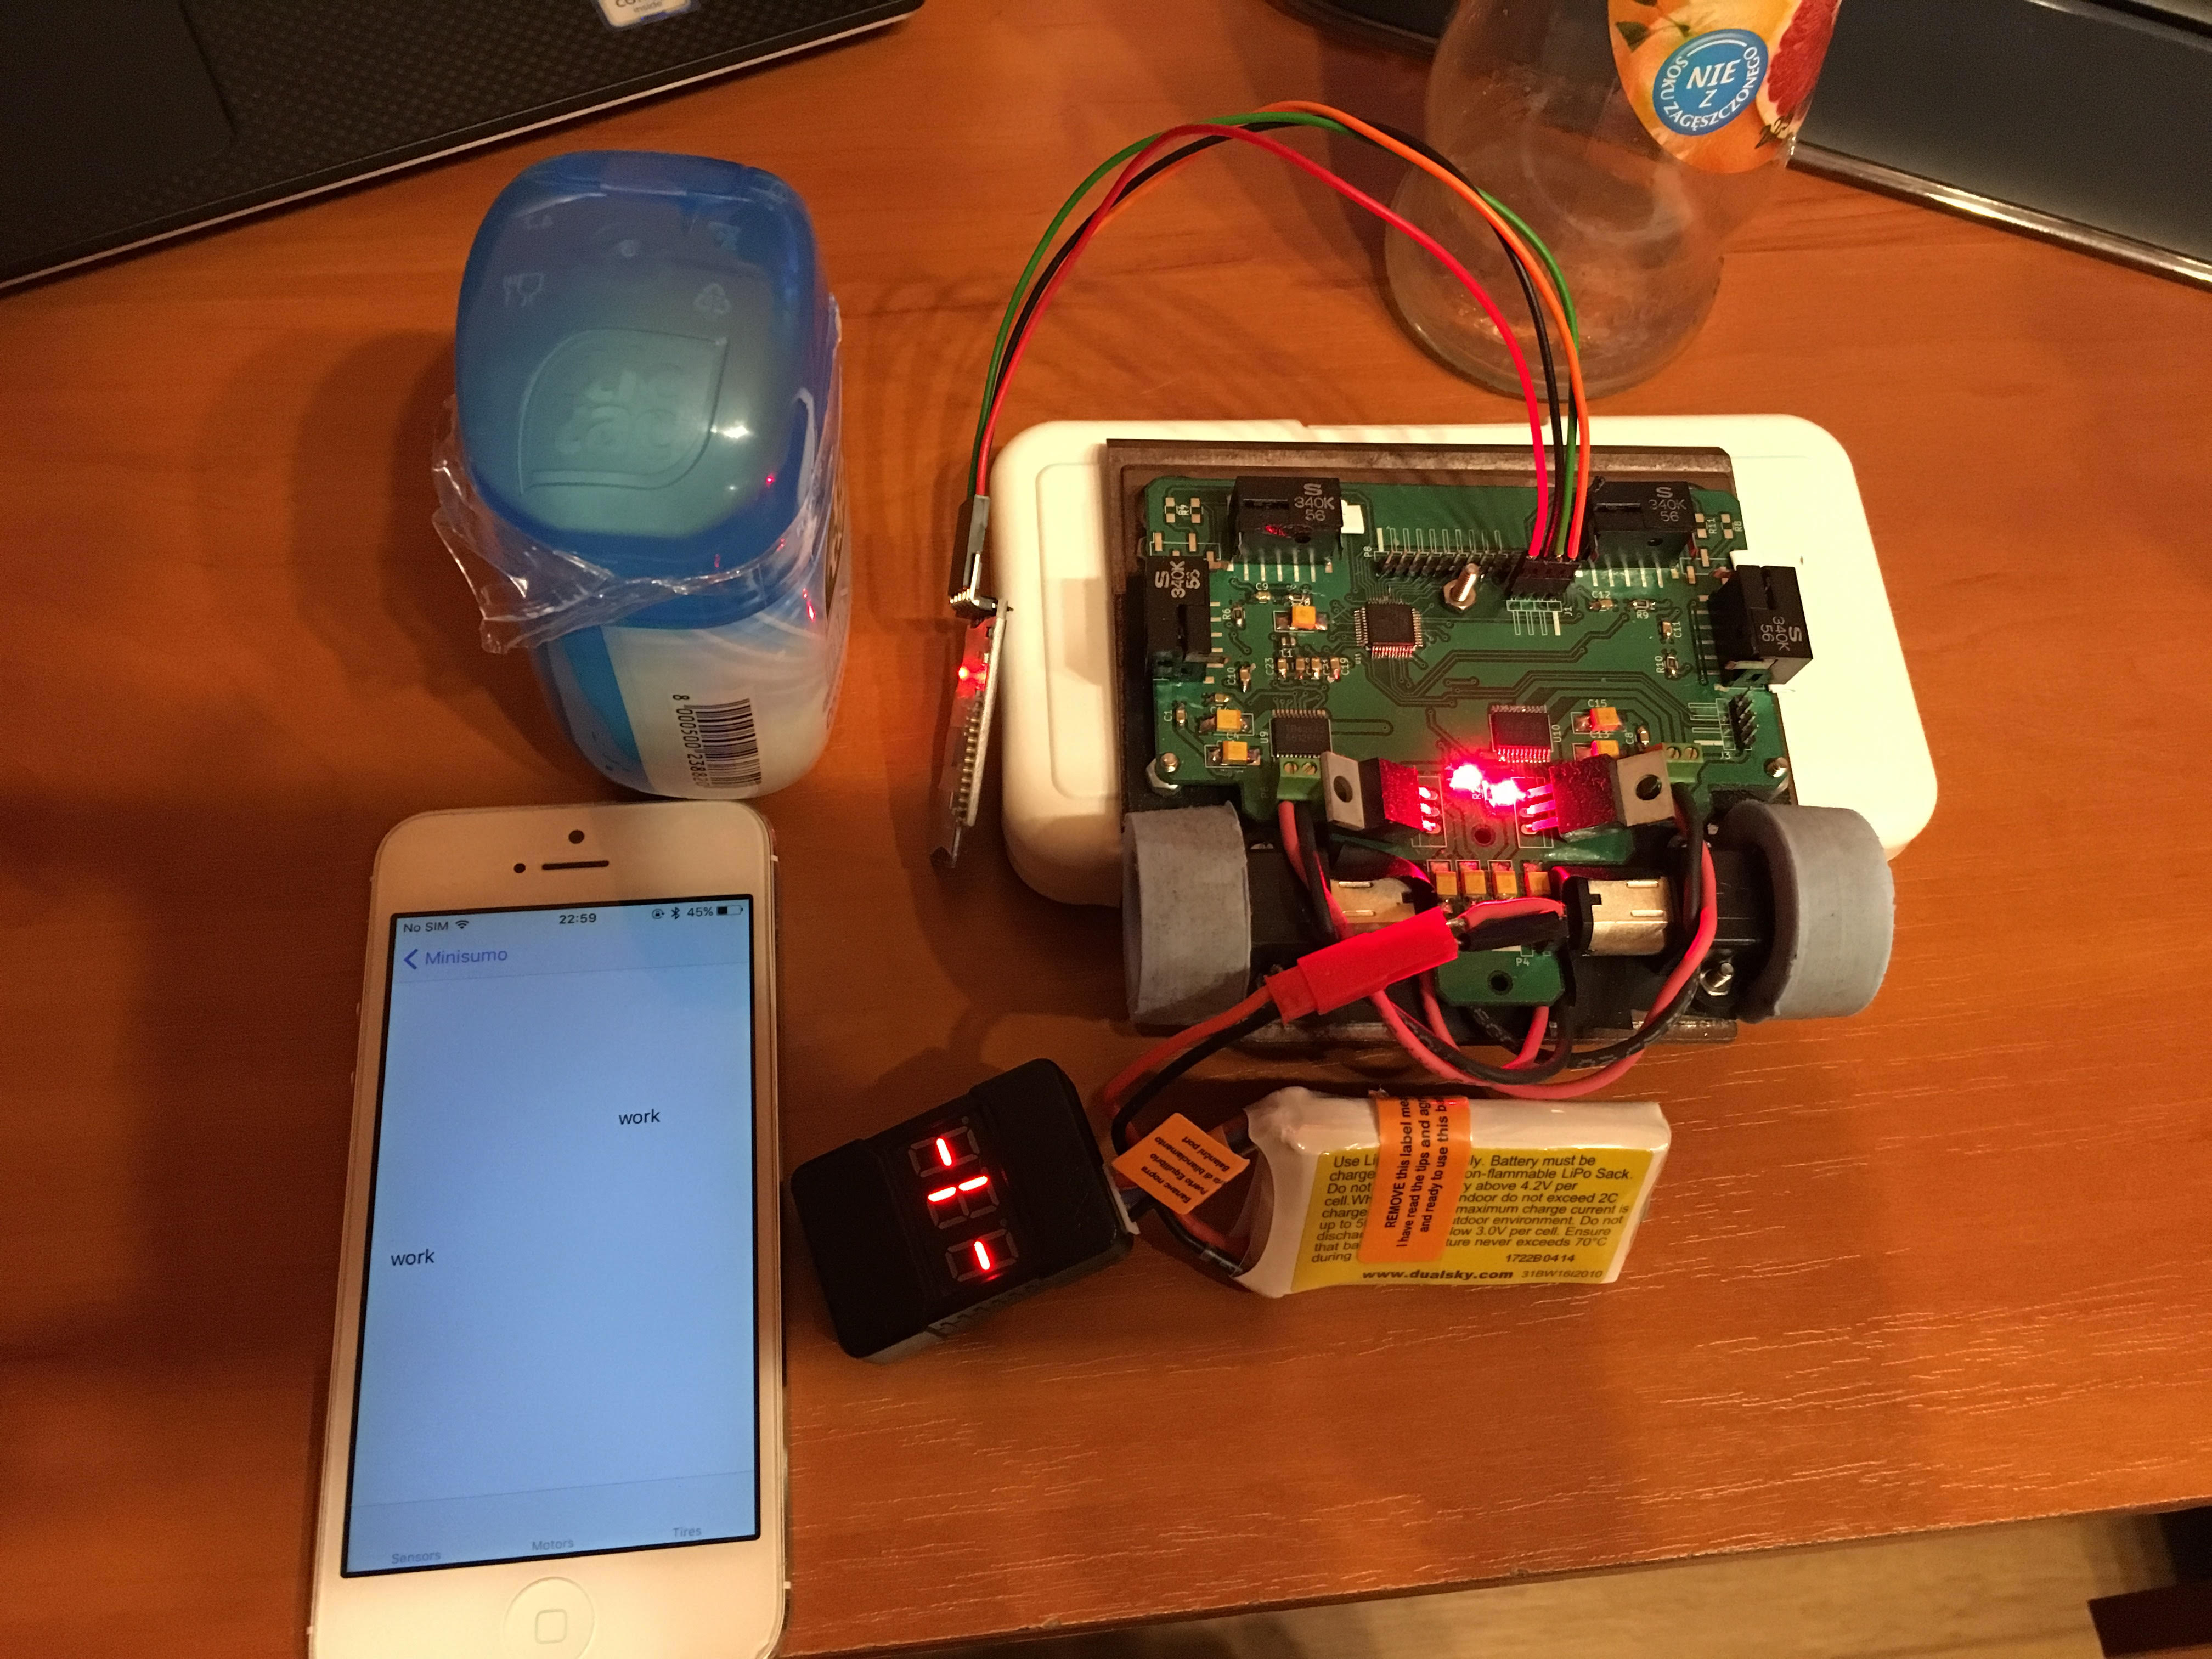
\includegraphics[width=0.75\linewidth]{pic05/sensorsvis.jpg}
	\caption{Poprawność działania diagnostyki czujników.}
	\label{fig:realsensors}	
\end{figure}

Natomiast na rysunku \ref{fig:realsensors} przedstawiono działanie omawianego panelu. Po lewej stronie znajduje się robot z zasłoniętym lewym oraz prawym górnym czujnikiem (oznacza to wykrycie przeciwnika), a po prawej stronie telefon z wizualizacją działania aplikacji. Jak widać wiadomość nadesłana z robota została odpowiednio zinterpretowana, ponieważ pojawiła się lewa oraz prawa górna etykieta \textit{work}.

\begin{minipage}{\textwidth}
	\begin{lstlisting}[label=sensors,caption=Parsowanie wiadomości zawierającej stan czujników.]
func parseSensors(state: String, label: UILabel) {
  if state == "1" {
    label.text = "work"
  } else {
    label.text = " "
  }
}
	\end{lstlisting}
\end{minipage}

Powyższy listing \ref{sensors} przedstawia funkcję \textit{parseSensors}, która ma na celu interpretację fragmentu wiadomości odnośnie stanu czujników nadesłanej przez robota. W przypadku otrzymania wartości 1 oznaczającej wykrycie przeciwnika pojawia się etykieta \textit{work}. W innych przypadkach etykieta jest niewidoczna.
 
\subsubsection{Diagnostyka silników}
Panel diagnostyki silników powstał w celu sprawdzenia zachowania poszczególnego motoru. Jego widok składa się z dwóch niezależnych suwaków, które służą do ustawienia odpowiedniej mocy oraz kierunku obrotu każdego z silników.

Rysunek \ref{fig:motors} przedstawia wygląd omawianego panelu. Domyślnie suwaki są wyśrodkowane, co oznacza brak obrotu. Przesunięcie suwaka w lewo powoduje ruch robota wstecz, natomiast w~prawo w przód.

\begin{figure}[H]
	\centering
		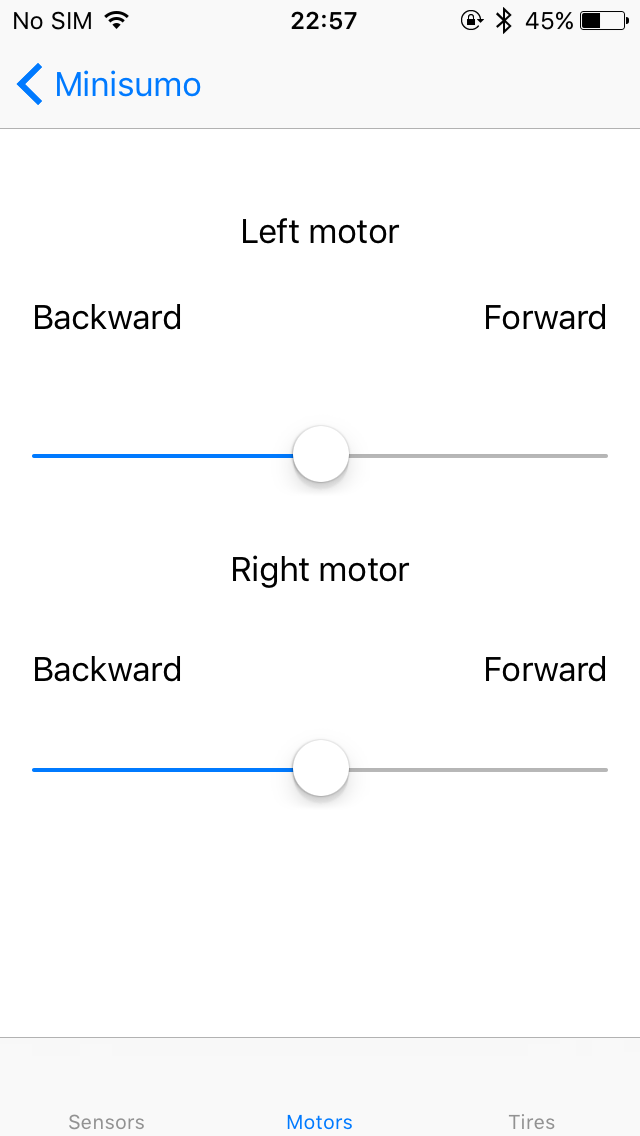
\includegraphics[width=0.75\linewidth, height=10cm, keepaspectratio, fbox]{pic05/motors.PNG}
	\caption{Widok diagnostyki silników.}
	\label{fig:motors}	
\end{figure}

Listing \ref{motorscode} zawiera implementację metody \textit{RightMotor} (należącej do klasy \textit{CheckMotorsViewController}), która nasłuchuje zmian położenia suwaka. Zakres wartości mieści się w przedziale od -100 do 100, gdzie wartości ujemne interpretowane są jako obrót silnika w tył (przeciwnie do ruchu wskazówek zegara). Linia 3 przedstawia pobranie wartości położenia suwaka. Linie 4 – 9 ukazują fragment kodu, który parsuje uzyskaną wartość i określa kierunek obrotu. Następnie wartość położenia suwaka jest parsowana na pojedyncze znaki oraz przypisywana do odpowiednich indeksów tablicy \textit{msg}, która zostaje wysłana do robota. Wiadomość z żądaną mocą oraz kierunkiem obrotu silnika wysyłana jest co 200 milisekund z powodów opisanych w~poprzednich podrozdziałach pracy. Analogicznie dla lewego silnika powstała metoda \textit{LeftMotor}.

\begin{minipage}{\textwidth}
	\begin{lstlisting}[label=motorscode,caption=Nasłuchiwanie zmiany położenia suwaka.]
IBAction func RightMotor(_ sender: UISlider) {
  
  rightMotorPower = Int(sender.value)
  if rightMotorPower < 0 {
    rightMotorDirection = 1
    rightMotorPower *= -1
  } else {
    rightMotorDirection = 2
  }
    
  msg[2] = String(rightMotorDirection)
    
  if rightMotorPower < 10 {
    msg[5] = "0"
    msg[6] = String(rightMotorPower)
  } else {
    msg[5] = String(rightMotorPower / 10)
    msg[6] = String(rightMotorPower % 10)
  }
    
  usleep(useconds_t(20 * ms))
  print(msg.joined())
  serial.sendMessageToDevice(msg.joined())
}
	\end{lstlisting}
\end{minipage}

\subsubsection{Czyszczenie opon}
Panel czyszczenia opon jest uboższą wersją panelu diagnostyki silników. Składa się z jednego przełącznika, który ustala moc obu silników na 20\% dostępnej mocy. Funkcjonalność powstała z~myślą o czyszczeniu opon robota, które wykonane zostały z poliuretanu przez co bardzo szybko tracą przyczepność z powodu dużej podatności na zbieranie brudu.

\newpage

Poniższy rysunek \ref{fig:tires} przedstawia wygląd panelu służącemu czyszczenia opon konstrukcji.

\begin{figure}[H]
	\centering
		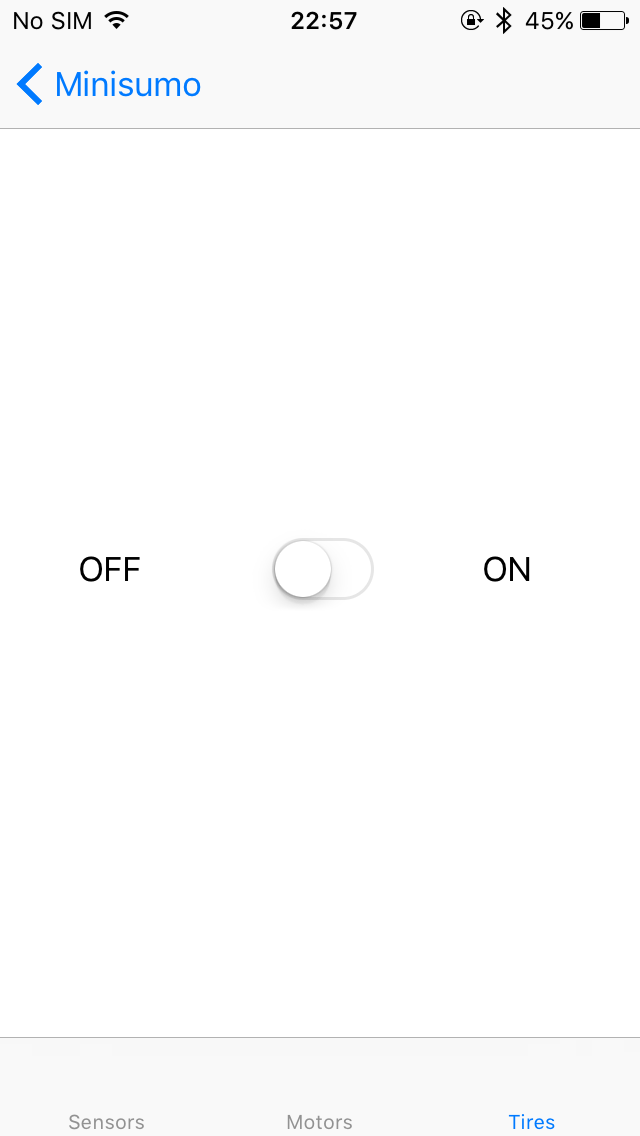
\includegraphics[width=0.75\linewidth, height=10cm, keepaspectratio, fbox]{pic05/tires.PNG}
	\caption{Widok funkcji czyszczenia opon.}
	\label{fig:tires}	
\end{figure}

Na listingu \ref{tirescode} przedstawiono metodę \textit{changedState} będącą członkiem klasy \textit{CleaningTiresViewController}. Wywoływana jest w momencie zmiany położenia przełącznika, a następnie w~zależności od jego stanu wysyła odpowiednio skonstruowaną wiadomość do robota.  

\begin{minipage}{\textwidth}
	\begin{lstlisting}[label=tirescode,caption=Nasłuchiwanie zmiany położenia przełącznika.]
IBAction func changedState(_ sender: UISwitch) {
  if sender.isOn {
    msg[0] = "3"
    serial.sendMessageToDevice(msg.joined())
  } else {
    msg[0] = "0"
    serial.sendMessageToDevice(msg.joined())
  }
}
	\end{lstlisting}
\end{minipage}

\newpage
 
\section{Kompilacja projektu}
Kompilacja projektu składa się z 2 etapów – kompilacji programu uruchamianego w robocie oraz aplikacji mobilnej. W celu wgrania oprogramowania robota należy skompilować kod źródłowy w środowisku \textit{Eclipse}, a następnie utworzony plik binarny przesłać do procesora pojazdu przy użyciu środowiska \textit{STMStudio}. Rozwiązanie nie należy do najwygodniejszych, szczególnie na etapie testowania. Niestety jest to jedyny sposób, wynikający z błędów popełnionych na etapie projektowania, które zostaną opisane w podsumowaniu. Drugi etap jest mniej problematyczny, ponieważ nie wymaga integracji oprogramowania z niededykowanym urządzeniem.  Kompilacja kodu aplikacji mobilnej odbywa się w obrębie jednego narzędzia jakim jest \textit{Xcode}. 


\chapter{Implementacja}

\section{Kompilacja projektu}

\chapter{Podsumowanie}
W pracy zaprojektowano oraz wykonano robota kategorii minisumo. Dodatkowo zaimplementowano aplikację mobilną na platformę iOS, która steruje wspomnianym robotem. Głównym założeniem powstałej aplikacji było umożliwienie wygodnego wyboru algorytmu walki bez potrzeby przeprogramowywania robota, bądź zawierania w projekcie elektroniki dodatkowych przycisków, które służyłyby przełączaniu funkcjonalności. Ponadto powstał panel diagnostyki czujników oraz silników, który okazał się nieoceniony, ponieważ użyty w pracy model czujników przeciwnika okazał się zawodny, czego z początku nie wzięto pod uwagę. W ramach pracy stworzono również możliwość sterowania zdalnego robotem. Funkcjonalność ta nie posiada większego zastosowania, aczkolwiek powstała w celach edukacyjnych. Warto zauważyć, iż cała aplikacja mobilna powstała w oparciu o wzorzec \textit{MVC}, dzięki czemu kod źródłowy jest łatwo modyfikowalny, a zastosowanie zrozumiałych nazw metod jak i zmiennych wpłynęło pozytywnie na czytelność kodu.

\section{Dalsze kierunki rozwoju projektu}
Do dalszych kierunków rozwoju należy:

\begin{itemize}
\item obsługę utraty połączenia \textit{Bluetooth} z robotem. Na chwilę obecną aplikacja w żaden sposób nie informuje użytkownika o braku łączności z urządzeniem docelowym. Wciąż jest responsywna, natomiast nie nadaje żadnych wiadomości;
\item możliwość tworzenia własnych algorytmów walki z poziomu aplikacji w oparciu o wcześniej zdefiniowane zachowania robota;
\item stworzenie panelu będącego dziennikiem odbytych zawodów wraz z możliwością sporządzania notatek;
\item obsługa czujników wykrywających koniec ringu;
\item poprawa złącza zasilania w robocie, ponieważ obecne pod wpływem drgań potrafi chwilowo przerwać zasilanie przez co następuje restart robota;
\item poprawa schematu elektroniki. Głównie ulepszenie filtracji zasilania perfyferiów oraz zlikwidowanie przelotek w ścieżkach między zasilaniem, a odbiornikiem, które prądowe zapotrzebowanie jest wysokie (mostki H będące sterownikami silników).
\item nawiercenie stalowego podwozia robota w celu zmniejszenia masy;
\item wykonanie trwalszego nadwozia;
\item zastosowanie mocniejszych sterowników silników w celu zwiększenia szansy na wygraną podczas starcia w zwarciu;
\item przeprojektowania złącza programatora, ponieważ obecne nie uwzględnia linii NRST potrzebnej do uruchomienia oprogramowania w trybie debugowania, przez co utrudnione jest wyszukiwanie potencjalnych błędów w kodzie. 
\end{itemize}



\bibliographystyle{plabbrv}

%UWAGA: bibliotekę referencji należy przygotować samemu. Dobrym do tego narzędziem jest JabRef.

%       Nazwę przygotowanej biblioteki wpisuje się poniżej bez rozszerzenia
%       (w tym przypadku jest to "dokumentacja.bib")

\chapterstyle{noNumbered}
\phantomsection % sets an anchor
\addcontentsline{toc}{chapter}{Indeks rzeczowy}
\printindex

\begin{thebibliography}{99}
	
  			\bibitem{Sumo}
	\emph{Robot klasy sumo}
  \url{https://en.wikipedia.org/wiki/Robot-sumo}
  (dostęp 09.11.2017).
  		
  			\bibitem{Minisumo}
	\emph{Zawody minisumo}
  \url{https://pl.wikipedia.org/wiki/Minisumo}
  (dostęp 09.11.2017).
  
    			\bibitem{Forbot}
	\emph{Kurs HAL}
  \url{https://forbot.pl/blog/kurs-stm32-f4-1-czas-poznac-hal-spis-}
  \url{tresci-kursu-id14114}  
  (dostęp 09.11.2017).
  	
\end{thebibliography}

\end{document}

